\documentclass{article}
\usepackage[T1]{fontenc}
\usepackage[utf8]{inputenc}
\usepackage{lmodern}
\usepackage[polish,shorthands=off]{babel}
\usepackage{graphicx}
\usepackage{siunitx}
\usepackage{multirow}
\usepackage{longtable}
\usepackage{hyperref}
\usepackage{float}
\usepackage{enumitem}

\usepackage{animate}
\usepackage{tikz}
\usetikzlibrary{lindenmayersystems}
\pgfdeclarelindenmayersystem{A}{%
  \symbol{F}{\pgflsystemstep=0.6\pgflsystemstep\pgflsystemdrawforward}
  \rule{A->F[+A][-A]}
}

\title{Sprawozdanie obliczenia naukowe\\Lista 5}
\author{Jakub Kowal}
\date{}
\begin{document}
\maketitle

\section*{Zapis macierzy}
\subsection*{Reprezentacja macierzy}
Macierze są przechowywane w strukturze \textbf{BlockMatrix} jako wektor bloków diagonalnych \textbf{As} oraz wektory bloków nad i poddiagonalnych \textbf{Cs} i \textbf{Bs}. Każdy blok ma rozmiar $l\times l$, a liczba bloków na diagonali to $v=\frac{n}{l}$. Dzięki temu możemy zmniejszyć użycie pamięci z O($n^{2}$) do O($3\times v\times l^{2}$), gdzie $v\times l$ daje nam n, więc otrzymujemy O($n\times l$). Biorąc pod uwagę, że l jest stałe możemy przyjąć O($n$) jako złożoność pamięciową.

Operacje odczytu i zapisu używają pomocniczych funkcji \textbf{matrix\_get} i \textbf{matrix\_put}, które zwracają lub ustawiają wartości w konkretnych blokach znając współrzędne w oryginalnej macierzy. Mają złożoność obliczeniową O($1$).

\section*{Eliminacja Gaussa}
\subsection*{Implementacja}
Implementacja funkcji \textbf{Gauss} przeprowadza eliminację tylko w obrębie zapisywanych bloków. Taka implementacja jest możliwa dzięki specyficznej naturze naszej macierzy, która oznacza, że nie mamy potrzeby ingerowania w puste pola poza blokami \textbf{A}, \textbf{B} i \textbf{C}. Dla każdego wiersza obliczany jest mnożnik $I$ (Nie ma potrzeby zapisywać w pamięci tych mnożników, więc korzystamy z pojedynczej zmiennej) i wykonywana jest aktualizacja elementów w blokach oraz wektora prawej strony $b$.

Dzięki specyficznej postaci macierzy algorytm ten może wykonywać się tylko na wartościach przechowywanych w blokach, ponieważ reszta i tak byłaby zerowana przez zera spoza bloków. Pozwala nam to niesamowicie obniżyć złożoność z O($n^{3}$) do O($n$), ale to zostanie wytłumaczone w późniejszych punktach.

\subsubsection*{Eliminacja Gaussa z pivotingiem}
Funkcja \textbf{Gauss\_pivot} działa tak jak funkcja \textbf{Gauss}, ale dodatkowo wyszukuje największy element w kolumnie w zakresie pivotowania (ograniczonym przez nasze bloki) i wykonuje zamianę wierszy za pomocą \textbf{matrix\_swap}. Wykonuje też zamianę danych w wektorze b.

\section*{Rozkład LU}
\subsection*{Implementacja}
Funkcja \textbf{LU} zamienia macierz w postać, w której dolna część (poniżej diagonalnej) zawiera współczynniki L (mnożniki w postaci zmiennej $I$), a górna część macierz U. W implementacji mnożniki zapisywane są w macierzy w miejscu pól, które były zerowane przez eliminację Gaussa. Jest to praktycznie jedyna różnica względem eliminacji Gaussa.

\subsection*{Rozkład LU z pivotingiem}
	Funkcja \textbf{LU\_pivot} wykonuje wyszukiwanie pivotu analogicznie do pivotingu w eliminacji Gaussa i zamiany wierszy (funkcja \textbf{matrix\_LU\_swap}, która operuje na szerszym zakresie indeksów niż zwykły \textbf{matrix\_swap}). Następnie zapisuje mnożniki i aktualizuje elementy macierzy oraz wektorze b.

\section*{Obliczanie}
\subsection*{Implementacja}
Funkcja \textbf{solve\_gauss} wykonuje obliczanie $x$ od $x_{n}$ do $x_{1}$ na macierzy w postaci po eliminacji Gaussa (przyjmuje macierz i wektor prawej strony). Na wykładzie zostało opisane to wzorem:
\begin{center}
  $x_{k}=\frac{b_{k}-\sum_{j=k+1}^{n}a_{kj}x_{j}}{a_{kk}}$
\end{center}
 Z kolei \textbf{solve\_LU} najpierw modyfikuje wektor b, żeby wziąć pod uwagę mnożniki, które w eliminacji Gaussa na bieżąco zmieniały b, a w rozkładzie LU dopiero teraz trzeba wziąć pod uwagę. Następnie wykonuje po prostu \textbf{solve\_gauss} dla części U.
 
\section*{Złożoność}
\subsection*{Złożoność czasowa}
Dla operacji ograniczonych do pasma szerokości z grubsza proporcjonalnej do $l$ (blok szerokości $l$) analizujemy koszt pojedynczego kroku $k$: pętle po $i$ i $j$ mają długość rzędu $O(l)$, zatem koszt dla danego $k$ to $O(l^2)$. Sumując po wszystkich $k=1\ldots n$ otrzymujemy złożoność
$$T(n)=O(n\,l^{2}).$$
Jeżeli $l$ jest stałe i małą wartością w stosunku do $n$, złożoność redukuje się praktycznie do $O(n)$ (linowa względem $n$).

W przeciwieństwie do pełnej eliminacji Gaussa na macierzach gęstych, która ma $O(n^{3})$, wykorzystanie struktury blokowej i ograniczonego pasma daje dużą oszczędność czasu.

\subsection*{Złożoność pamięciowa}
Macierz jest przechowywana jako $v= n/l$ bloków rozmiaru $l\times l$, stąd pamięć zajęta przez bloki diagonalne to $v\cdot l^{2}=n\,l$. Podobnie bloki nad- i poddiagonalne też razem dają rząd $O(n\,l)$. Wektory prawej strony i rozwiązania są długości $n$. Zatem całkowite wymagania pamięciowe to
$$M(n)=O(n\,l).$$
Dla stałego i małego $l$ jest to liniowe w $n$, znacząco mniej niż $O(n^{2})$ dla pełnej macierzy gęstej.

\section*{Wyniki i wnioski}
W pliku z eksperymentami (\textbf{Usage.jl}) wykonane zostały pomiary czasu i alokacji pamięci dla czterech wariantów: \textbf{Gauss}, \textbf{Gauss Pivot}, \textbf{LU} i \textbf{LU Pivot}. Wykresy wyników zostały dołączone jako \textbf{time\_graph.png} i \textbf{mem\_graph.png}.

Obserwacje istotne dla wniosków:
- Implementacje operują wewnątrz bloku/pasma, stąd złożoność rośnie liniowo z $n$ mnożoną przez $l^{2}$, a nie jak $n^{3}$.
- \textbf{LU} zapisuje mnożniki L w macierzy (dolna trójkątna część jest wypełniana wartościami różnymi od zera), co zmienia strukturę danych po obliczeniach w porównaniu do \textbf{Gauss}, który ustawia część eliminowaną na zera. W praktyce jednak pamięć bloków jest wcześniej zaalokowana, więc różnica pamięci bezpośrednio po operacji zależy od dodatkowych alokacji pomocniczych.
- Wpływ pivotingu: pivoting wymusza dodatkowe zamiany wierszy ( funkcje \textbf{matrix\_swap} i \textbf{matrix\_LU\_swap} ), co zwiększa liczbę odczytów/zapisów i nieznacznie narzut czasowy; \textbf{matrix\_LU\_swap} operuje na nieco szerszym zakresie indeksów, co zwiększa koszty przy pivotingu w LU.

Propozycje optymalizacji i uwagi metodyczne:
- Jeżeli chcemy minimalizować alokacje, należy unikać kopiowania wektora w funkcjach rozwiązujących — w aktualnej wersji \textbf{solve\_LU} modyfikacja wektora jest wykonywana in-place (komentarz z \textbf{y = copy(b)} został zakomentowany), co redukuje jedną dużą alokację.
- Dla stabilniejszych i powtarzalnych pomiarów rekomenduję użycie pakietu \textbf{BenchmarkTools.@btime} zamiast \textbf{@timed} — daje lepsze statystyki alokacji i czasu.
- Można też ograniczyć zwroty z \textbf{matrix\_put} (nie musi zwracać macierzy), aby zmniejszyć narzut wywołań funkcyjnych.


\section*{Wyniki}
\subsection*{Wyniki czasowe}
\begin{figure}[H]
    \label{fig:times}
    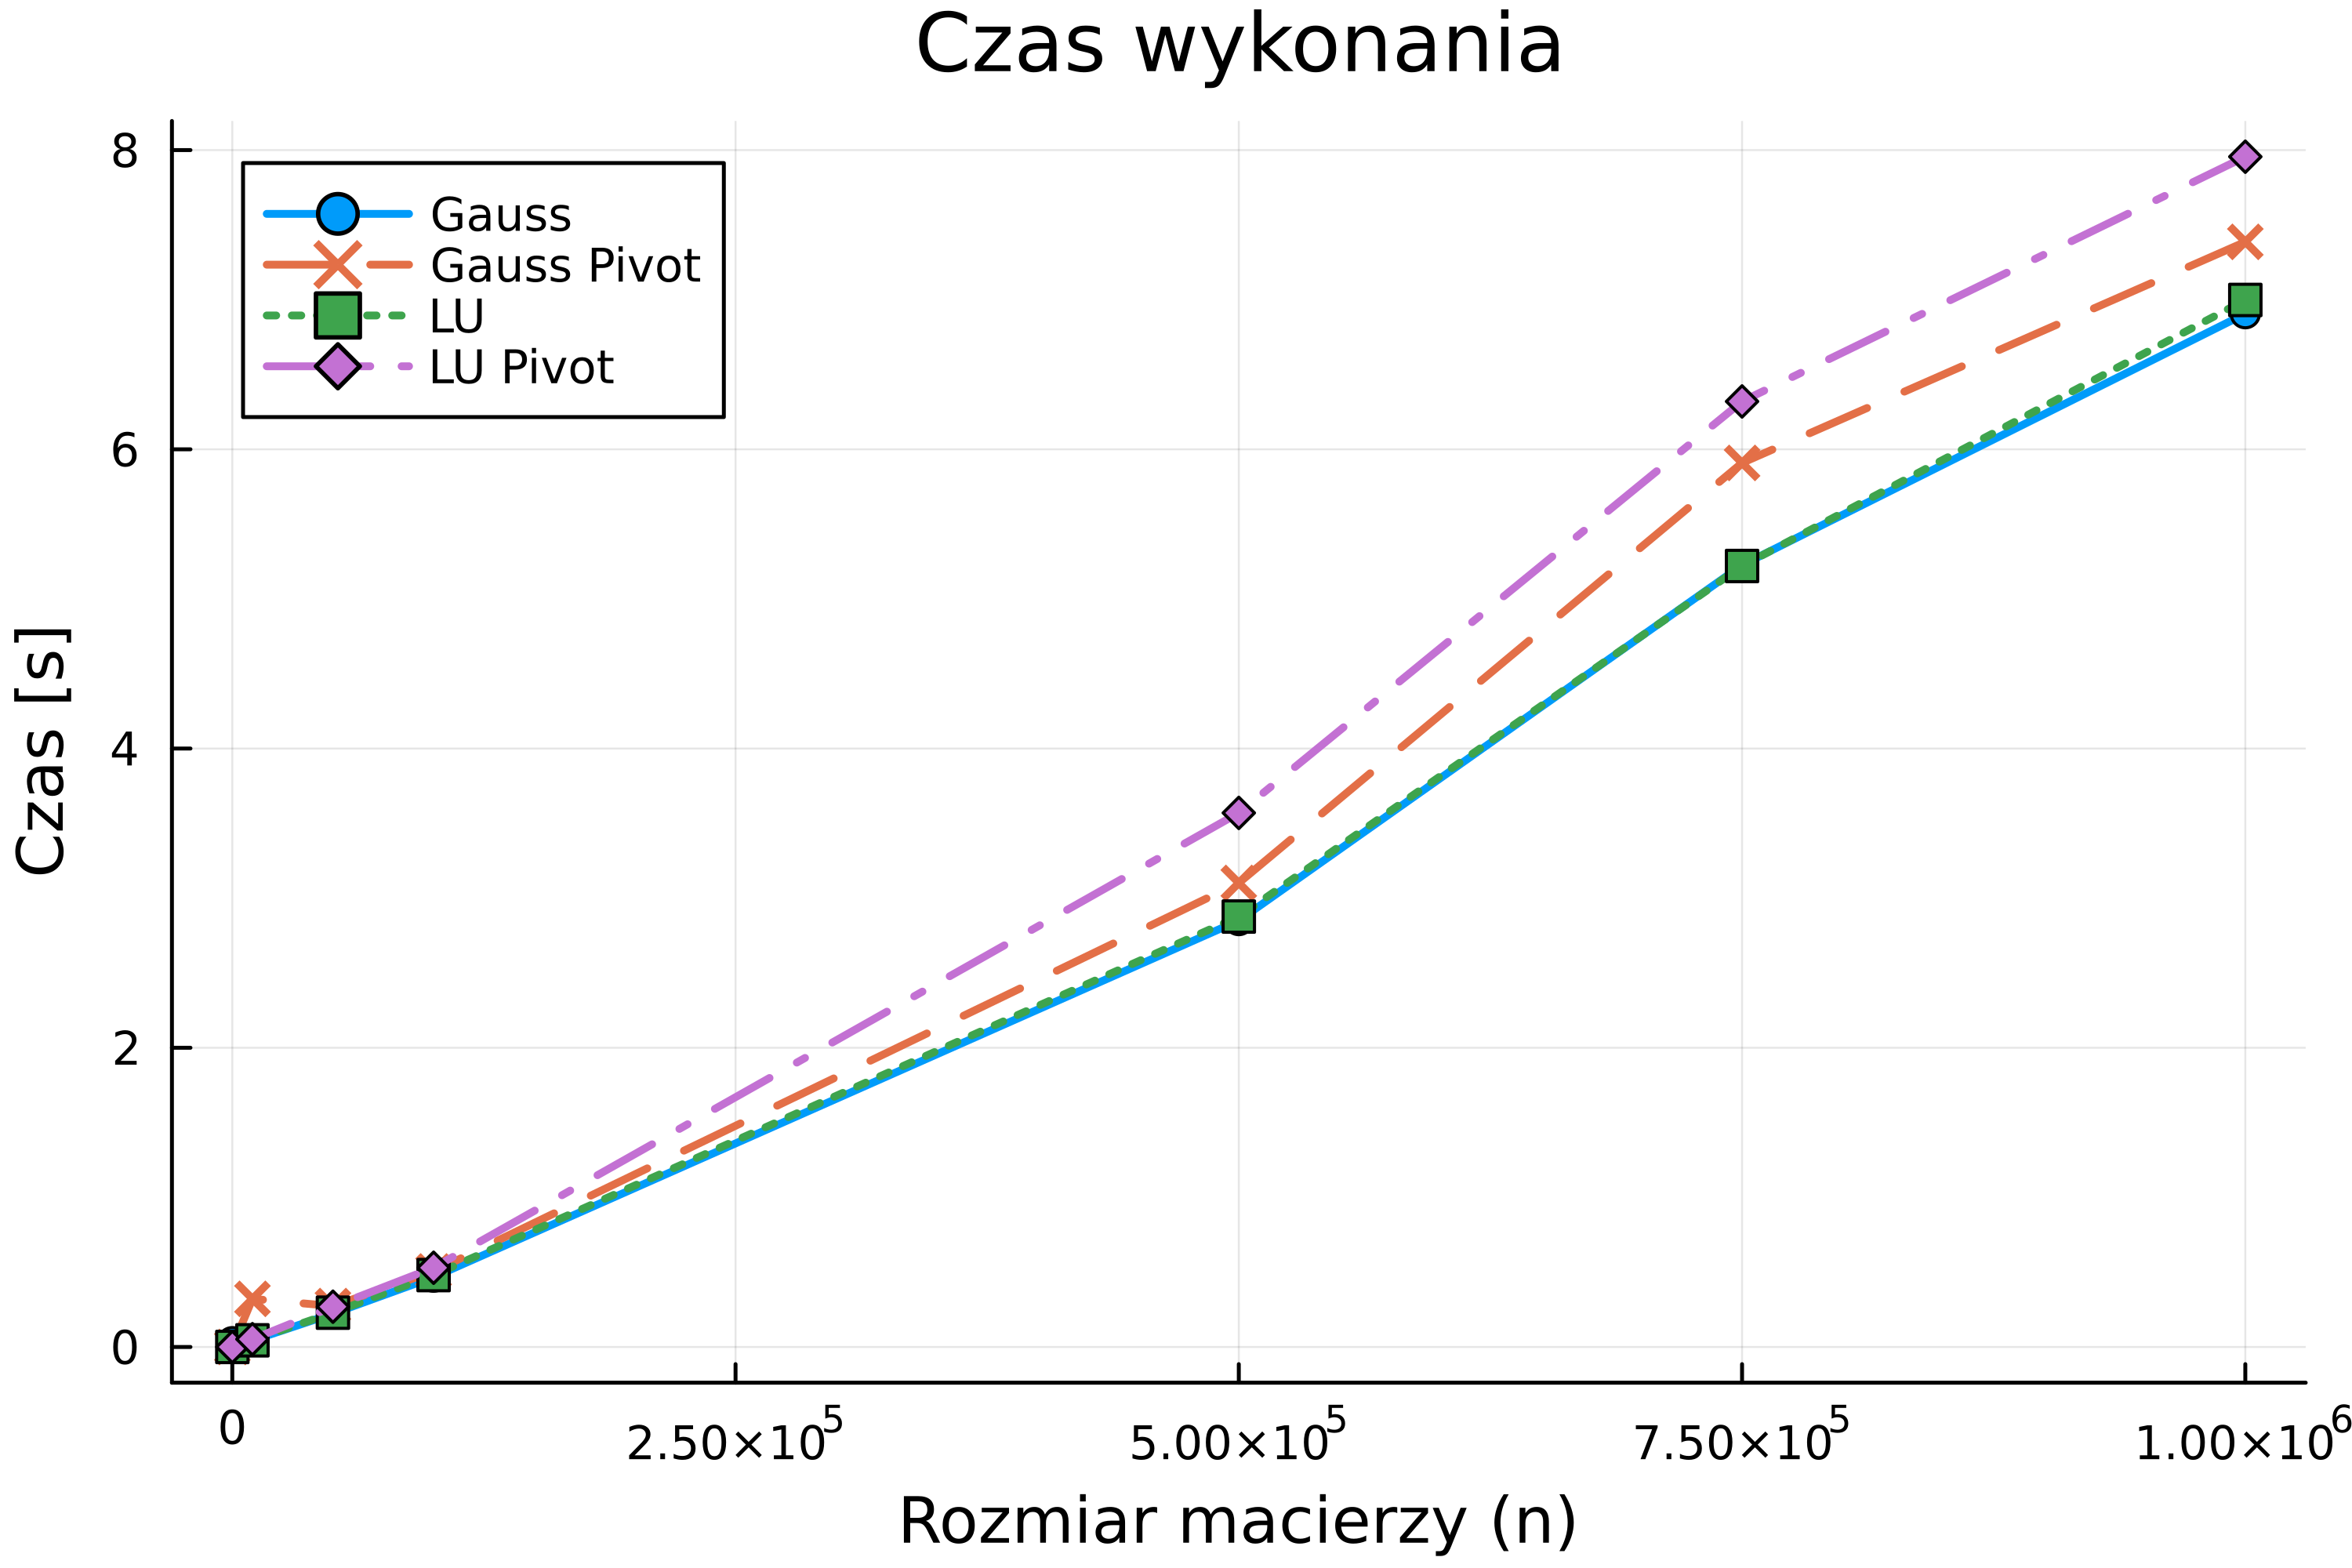
\includegraphics[width=35em]{time_graph.png}
\end{figure}
\subsection*{Wyniki pamięciowe}
\begin{figure}[H]
    \label{fig:memory}
    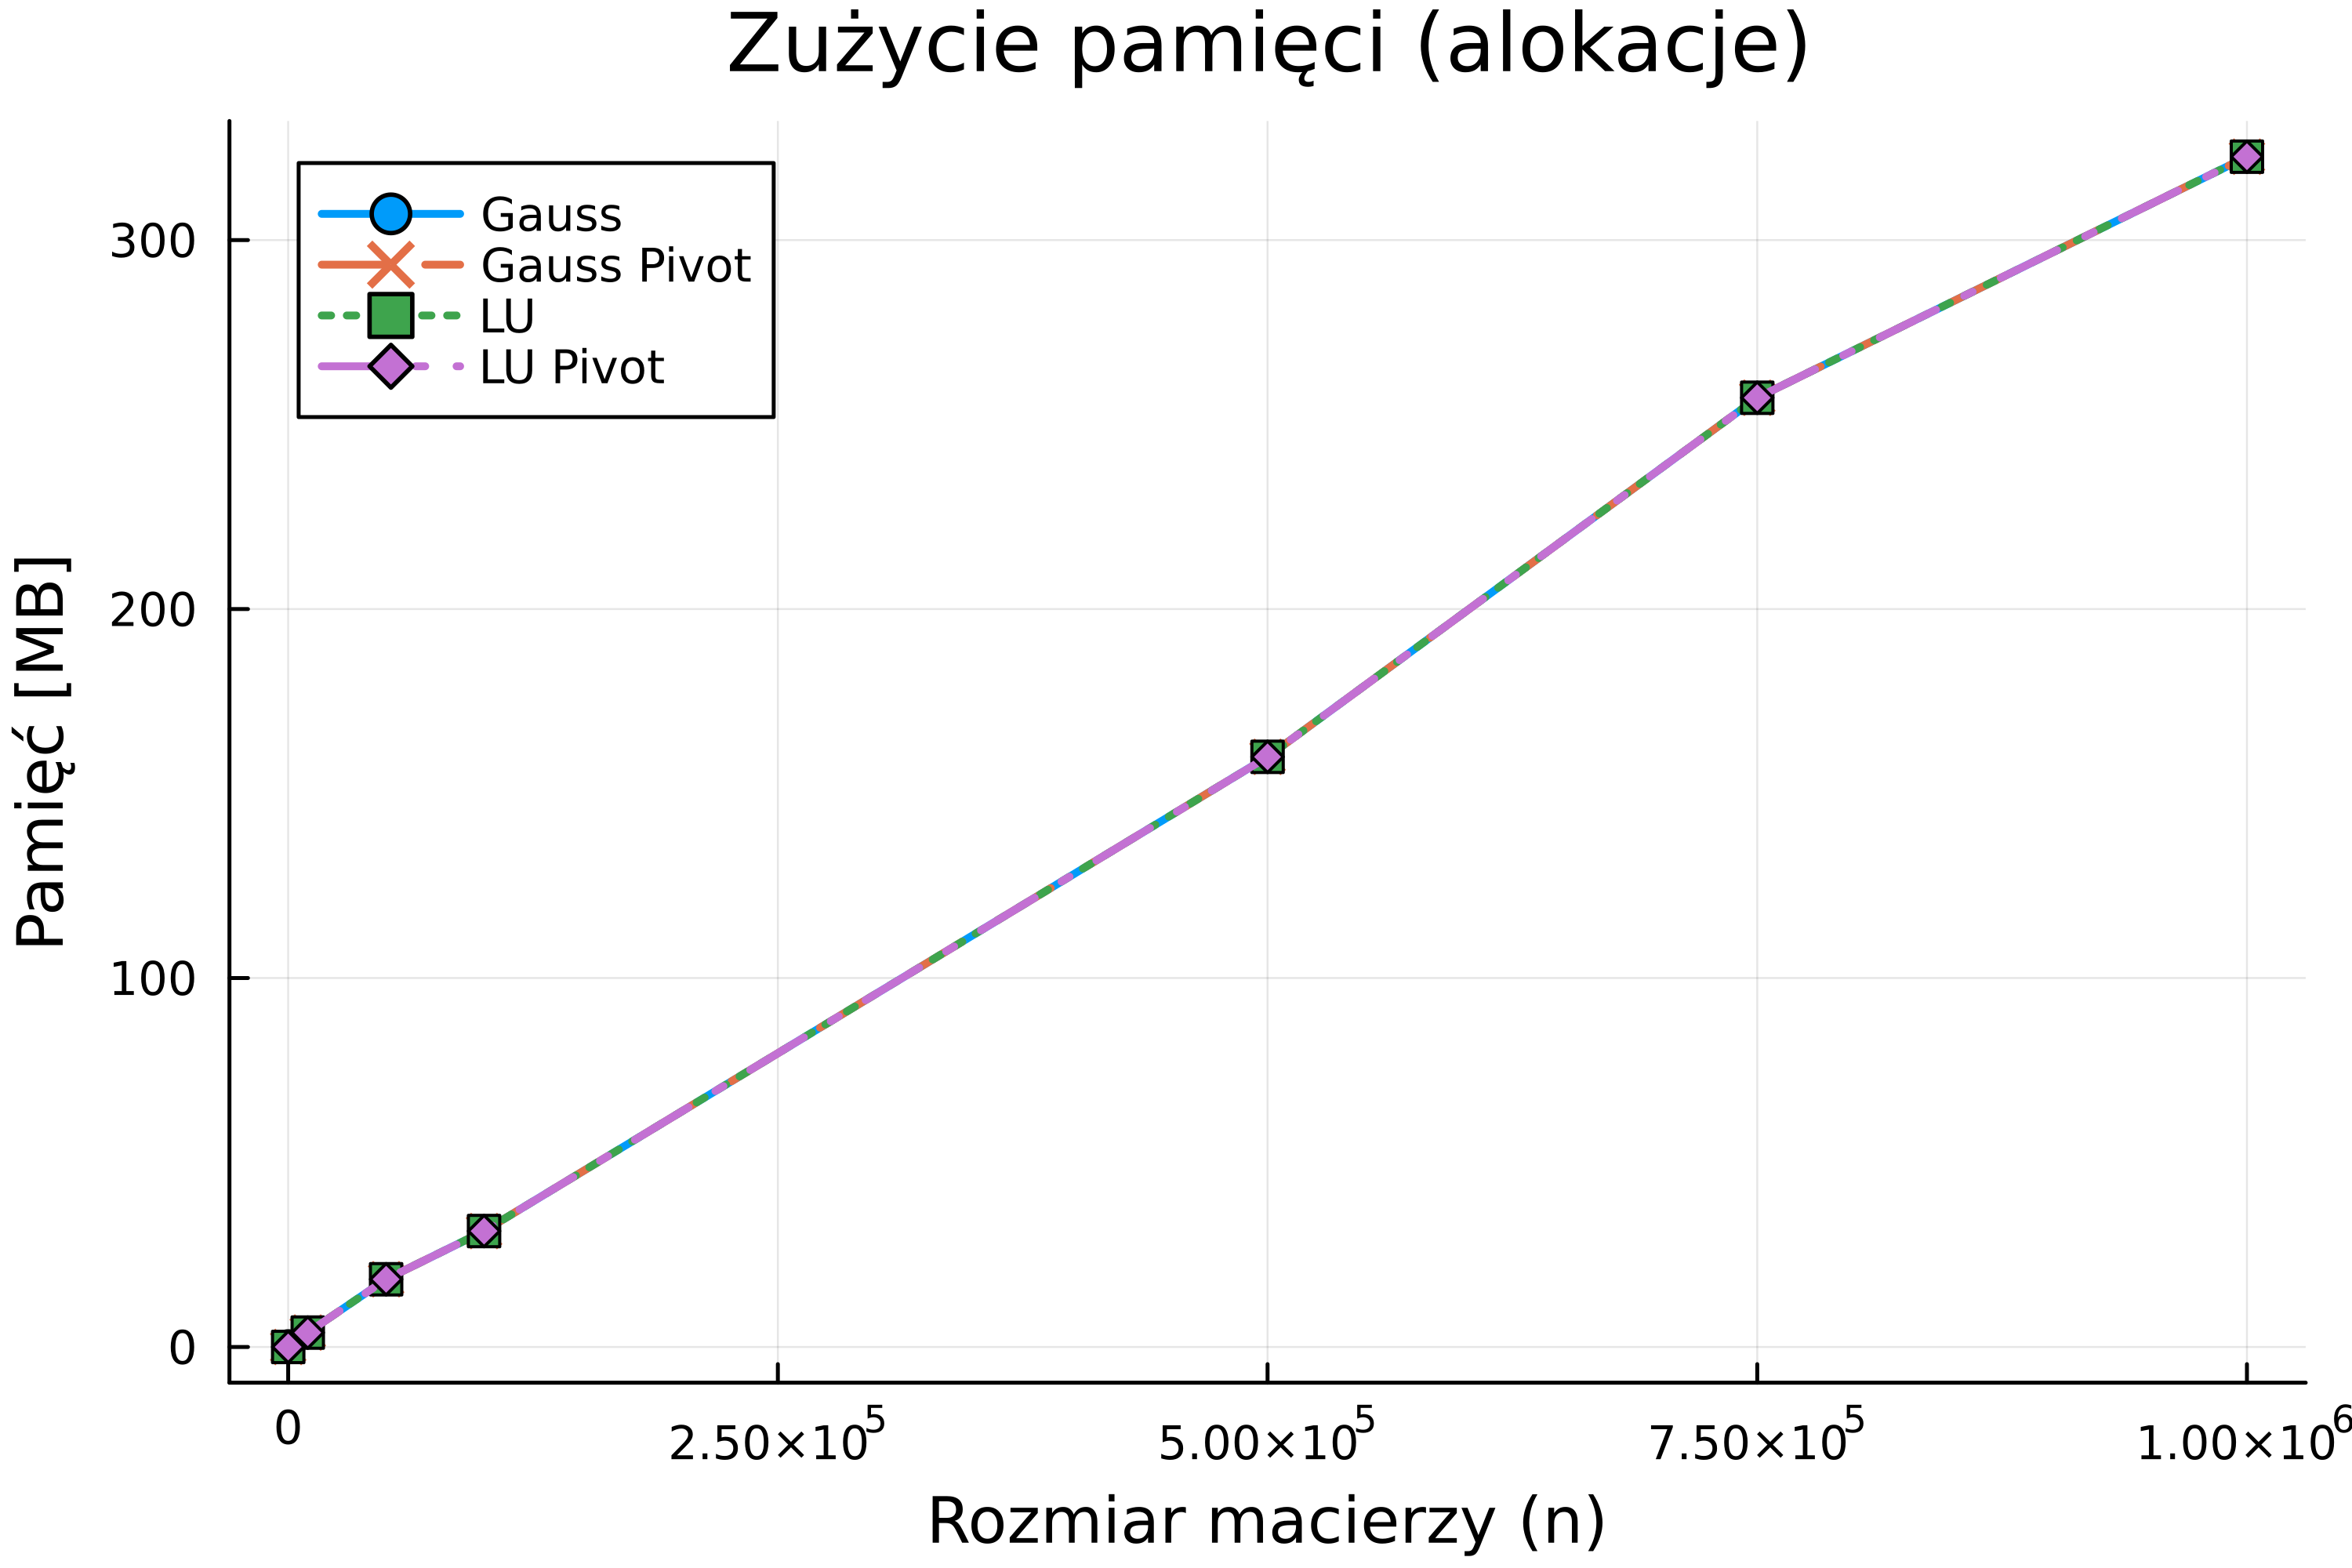
\includegraphics[width=35em]{mem_graph.png}
\end{figure}

\section*{Wnioski}
Algorytmy korzystają z reprezentacji blokowej, co pozwala na istotne przyspieszenie i ograniczenie pamięci w porównaniu do pełnej macierzy. Dzięki stałemu l koszty są asymptotycznie rzędu O($n$) w czasie i O($n$) w pamięci, co czyni podejście niesamowicie efektywnym dla dużych $n$.

\section*{Ciekawostka}
Tą animację wygenerował ChatGPT wykorzystując pakiet animate oraz tikz. Do generowania kolejnych klatek użył osobnego skryptu pythonowego.\\

\begin{animateinline}[controls,autoplay,loop, poster=first]{2}
\begin{tikzpicture}[scale=0.4, yscale=-1]
\draw[step=1cm,gray!20,very thin] (0,0) grid (16,16);
\fill[black] (9,11) rectangle (10,12);
\fill[black] (6,2) rectangle (7,3);
\fill[black] (3,4) rectangle (4,5);
\fill[black] (0,4) rectangle (1,5);
\fill[black] (15,13) rectangle (16,14);
\fill[black] (12,13) rectangle (13,14);
\fill[black] (7,8) rectangle (8,9);
\fill[black] (5,7) rectangle (6,8);
\fill[black] (1,1) rectangle (2,2);
\fill[black] (11,9) rectangle (12,10);
\fill[black] (10,12) rectangle (11,13);
\fill[black] (10,10) rectangle (11,11);
\fill[black] (3,6) rectangle (4,7);
\fill[black] (15,15) rectangle (16,16);
\fill[black] (13,14) rectangle (14,15);
\fill[black] (12,15) rectangle (13,16);
\fill[black] (7,5) rectangle (8,6);
\fill[black] (1,3) rectangle (2,4);
\fill[black] (11,11) rectangle (12,12);
\fill[black] (5,4) rectangle (6,5);
\fill[black] (7,3) rectangle (8,4);
\fill[black] (2,4) rectangle (3,5);
\fill[black] (14,13) rectangle (15,14);
\fill[black] (9,8) rectangle (10,9);
\fill[black] (7,7) rectangle (8,8);
\fill[black] (3,1) rectangle (4,2);
\fill[black] (1,0) rectangle (2,1);
\fill[black] (0,1) rectangle (1,2);
\fill[black] (13,9) rectangle (14,10);
\fill[black] (9,12) rectangle (10,13);
\fill[black] (3,5) rectangle (4,6);
\fill[black] (15,14) rectangle (16,15);
\fill[black] (14,12) rectangle (15,13);
\fill[black] (14,15) rectangle (15,16);
\fill[black] (9,5) rectangle (10,6);
\fill[black] (1,2) rectangle (2,3);
\fill[black] (0,3) rectangle (1,4);
\fill[black] (4,4) rectangle (5,5);
\fill[black] (3,7) rectangle (4,8);
\fill[black] (11,8) rectangle (12,9);
\fill[black] (8,10) rectangle (9,11);
\fill[black] (3,0) rectangle (4,1);
\fill[black] (2,1) rectangle (3,2);
\fill[black] (14,10) rectangle (15,11);
\fill[black] (11,12) rectangle (12,13);
\fill[black] (5,5) rectangle (6,6);
\fill[black] (4,6) rectangle (5,7);
\fill[black] (14,14) rectangle (15,15);
\fill[black] (3,2) rectangle (4,3);
\fill[black] (2,3) rectangle (3,4);
\fill[black] (0,2) rectangle (1,3);
\fill[black] (15,11) rectangle (16,12);
\fill[black] (6,4) rectangle (7,5);
\fill[black] (4,8) rectangle (5,9);
\fill[black] (11,7) rectangle (12,8);
\fill[black] (8,9) rectangle (9,10);
\fill[black] (10,8) rectangle (11,9);
\fill[black] (7,10) rectangle (8,11);
\fill[black] (2,0) rectangle (3,1);
\fill[black] (13,12) rectangle (14,13);
\fill[black] (6,6) rectangle (7,7);
\fill[black] (4,5) rectangle (5,6);
\fill[black] (8,11) rectangle (9,12);
\fill[black] (2,2) rectangle (3,3);
\fill[black] (11,13) rectangle (12,14);
\fill[black] (8,4) rectangle (9,5);
\fill[black] (6,8) rectangle (7,9);
\fill[black] (4,7) rectangle (5,8);
\fill[black] (10,9) rectangle (11,10);
\fill[black] (12,8) rectangle (13,9);
\fill[black] (9,10) rectangle (10,11);
\fill[black] (7,9) rectangle (8,10);
\fill[black] (4,0) rectangle (5,1);
\fill[black] (15,12) rectangle (16,13);
\fill[black] (12,14) rectangle (13,15);
\fill[black] (11,15) rectangle (12,16);
\fill[black] (12,12) rectangle (13,13);
\fill[black] (6,5) rectangle (7,6);
\fill[black] (5,6) rectangle (6,7);
\fill[black] (10,11) rectangle (11,12);
\fill[black] (7,11) rectangle (8,12);
\fill[black] (1,4) rectangle (2,5);
\fill[black] (3,3) rectangle (4,4);
\fill[black] (13,13) rectangle (14,14);
\fill[black] (8,8) rectangle (9,9);
\fill[black] (7,4) rectangle (8,5);
\fill[black] (6,7) rectangle (7,8);
\fill[black] (0,0) rectangle (1,1);
\fill[black] (5,8) rectangle (6,9);
\fill[black] (11,14) rectangle (12,15);
\fill[black] (11,10) rectangle (12,11);
\fill[black] (9,9) rectangle (10,10);
\fill[black] (8,12) rectangle (9,13);
\fill[black] (5,1) rectangle (6,2);
\fill[black] (13,15) rectangle (14,16);
\fill[black] (10,6) rectangle (11,7);
\fill[black] (7,6) rectangle (8,7);
\end{tikzpicture}
\newframe
\begin{tikzpicture}[scale=0.4, yscale=-1]
\draw[step=1cm,gray!20,very thin] (0,0) grid (16,16);
\fill[black] (9,11) rectangle (10,12);
\fill[black] (6,2) rectangle (7,3);
\fill[black] (3,4) rectangle (4,5);
\fill[orange] (0,4) rectangle (1,5);
\fill[black] (15,13) rectangle (16,14);
\fill[black] (12,13) rectangle (13,14);
\fill[black] (7,8) rectangle (8,9);
\fill[black] (5,7) rectangle (6,8);
\fill[black] (1,1) rectangle (2,2);
\fill[black] (11,9) rectangle (12,10);
\fill[black] (10,12) rectangle (11,13);
\fill[black] (10,10) rectangle (11,11);
\fill[black] (3,6) rectangle (4,7);
\fill[black] (15,15) rectangle (16,16);
\fill[black] (13,14) rectangle (14,15);
\fill[black] (12,15) rectangle (13,16);
\fill[black] (7,5) rectangle (8,6);
\fill[black] (1,3) rectangle (2,4);
\fill[black] (11,11) rectangle (12,12);
\fill[black] (5,4) rectangle (6,5);
\fill[black] (7,3) rectangle (8,4);
\fill[black] (2,4) rectangle (3,5);
\fill[black] (14,13) rectangle (15,14);
\fill[black] (9,8) rectangle (10,9);
\fill[black] (7,7) rectangle (8,8);
\fill[black] (3,1) rectangle (4,2);
\fill[black] (1,0) rectangle (2,1);
\fill[orange] (0,1) rectangle (1,2);
\fill[black] (13,9) rectangle (14,10);
\fill[black] (9,12) rectangle (10,13);
\fill[black] (3,5) rectangle (4,6);
\fill[black] (15,14) rectangle (16,15);
\fill[black] (14,12) rectangle (15,13);
\fill[black] (14,15) rectangle (15,16);
\fill[black] (9,5) rectangle (10,6);
\fill[black] (1,2) rectangle (2,3);
\fill[orange] (0,3) rectangle (1,4);
\fill[black] (4,4) rectangle (5,5);
\fill[black] (3,7) rectangle (4,8);
\fill[black] (11,8) rectangle (12,9);
\fill[black] (8,10) rectangle (9,11);
\fill[black] (3,0) rectangle (4,1);
\fill[black] (2,1) rectangle (3,2);
\fill[black] (14,10) rectangle (15,11);
\fill[black] (11,12) rectangle (12,13);
\fill[black] (5,5) rectangle (6,6);
\fill[black] (4,6) rectangle (5,7);
\fill[black] (14,14) rectangle (15,15);
\fill[black] (3,2) rectangle (4,3);
\fill[black] (2,3) rectangle (3,4);
\fill[orange] (0,2) rectangle (1,3);
\fill[black] (15,11) rectangle (16,12);
\fill[black] (6,4) rectangle (7,5);
\fill[black] (4,8) rectangle (5,9);
\fill[black] (11,7) rectangle (12,8);
\fill[black] (8,9) rectangle (9,10);
\fill[black] (10,8) rectangle (11,9);
\fill[black] (7,10) rectangle (8,11);
\fill[black] (2,0) rectangle (3,1);
\fill[black] (13,12) rectangle (14,13);
\fill[black] (6,6) rectangle (7,7);
\fill[black] (4,5) rectangle (5,6);
\fill[black] (8,11) rectangle (9,12);
\fill[black] (2,2) rectangle (3,3);
\fill[black] (11,13) rectangle (12,14);
\fill[black] (8,4) rectangle (9,5);
\fill[black] (6,8) rectangle (7,9);
\fill[black] (4,7) rectangle (5,8);
\fill[black] (10,9) rectangle (11,10);
\fill[black] (12,8) rectangle (13,9);
\fill[black] (9,10) rectangle (10,11);
\fill[black] (7,9) rectangle (8,10);
\fill[black] (4,0) rectangle (5,1);
\fill[black] (15,12) rectangle (16,13);
\fill[black] (12,14) rectangle (13,15);
\fill[black] (11,15) rectangle (12,16);
\fill[black] (12,12) rectangle (13,13);
\fill[black] (6,5) rectangle (7,6);
\fill[black] (5,6) rectangle (6,7);
\fill[black] (10,11) rectangle (11,12);
\fill[black] (7,11) rectangle (8,12);
\fill[black] (1,4) rectangle (2,5);
\fill[black] (3,3) rectangle (4,4);
\fill[black] (13,13) rectangle (14,14);
\fill[black] (8,8) rectangle (9,9);
\fill[black] (7,4) rectangle (8,5);
\fill[black] (6,7) rectangle (7,8);
\fill[red] (0,0) rectangle (1,1);
\fill[black] (5,8) rectangle (6,9);
\fill[black] (11,14) rectangle (12,15);
\fill[black] (11,10) rectangle (12,11);
\fill[black] (9,9) rectangle (10,10);
\fill[black] (8,12) rectangle (9,13);
\fill[black] (5,1) rectangle (6,2);
\fill[black] (13,15) rectangle (14,16);
\fill[black] (10,6) rectangle (11,7);
\fill[black] (7,6) rectangle (8,7);
\end{tikzpicture}
\newframe
\begin{tikzpicture}[scale=0.4, yscale=-1]
\draw[step=1cm,gray!20,very thin] (0,0) grid (16,16);
\fill[black] (9,11) rectangle (10,12);
\fill[black] (6,2) rectangle (7,3);
\fill[black] (3,4) rectangle (4,5);
\fill[black] (15,13) rectangle (16,14);
\fill[black] (12,13) rectangle (13,14);
\fill[black] (7,8) rectangle (8,9);
\fill[black] (5,7) rectangle (6,8);
\fill[red] (1,1) rectangle (2,2);
\fill[black] (11,9) rectangle (12,10);
\fill[black] (10,12) rectangle (11,13);
\fill[black] (10,10) rectangle (11,11);
\fill[black] (3,6) rectangle (4,7);
\fill[orange] (1,5) rectangle (2,6);
\fill[black] (15,15) rectangle (16,16);
\fill[black] (13,14) rectangle (14,15);
\fill[black] (12,15) rectangle (13,16);
\fill[black] (7,5) rectangle (8,6);
\fill[orange] (1,3) rectangle (2,4);
\fill[black] (11,11) rectangle (12,12);
\fill[black] (5,4) rectangle (6,5);
\fill[black] (7,3) rectangle (8,4);
\fill[black] (2,4) rectangle (3,5);
\fill[orange] (1,7) rectangle (2,8);
\fill[black] (14,13) rectangle (15,14);
\fill[black] (9,8) rectangle (10,9);
\fill[black] (7,7) rectangle (8,8);
\fill[black] (3,1) rectangle (4,2);
\fill[black] (1,0) rectangle (2,1);
\fill[black] (13,9) rectangle (14,10);
\fill[black] (9,12) rectangle (10,13);
\fill[black] (3,5) rectangle (4,6);
\fill[black] (2,6) rectangle (3,7);
\fill[black] (15,14) rectangle (16,15);
\fill[black] (14,12) rectangle (15,13);
\fill[black] (14,15) rectangle (15,16);
\fill[black] (9,5) rectangle (10,6);
\fill[orange] (1,2) rectangle (2,3);
\fill[black] (4,4) rectangle (5,5);
\fill[black] (3,7) rectangle (4,8);
\fill[black] (11,8) rectangle (12,9);
\fill[black] (8,10) rectangle (9,11);
\fill[black] (3,0) rectangle (4,1);
\fill[black] (2,1) rectangle (3,2);
\fill[black] (14,10) rectangle (15,11);
\fill[black] (11,12) rectangle (12,13);
\fill[black] (5,5) rectangle (6,6);
\fill[black] (4,6) rectangle (5,7);
\fill[black] (2,5) rectangle (3,6);
\fill[black] (14,14) rectangle (15,15);
\fill[black] (3,2) rectangle (4,3);
\fill[black] (2,3) rectangle (3,4);
\fill[black] (15,11) rectangle (16,12);
\fill[black] (6,4) rectangle (7,5);
\fill[black] (4,8) rectangle (5,9);
\fill[black] (2,7) rectangle (3,8);
\fill[black] (11,7) rectangle (12,8);
\fill[black] (8,9) rectangle (9,10);
\fill[black] (10,8) rectangle (11,9);
\fill[black] (7,10) rectangle (8,11);
\fill[black] (4,1) rectangle (5,2);
\fill[black] (2,0) rectangle (3,1);
\fill[black] (13,12) rectangle (14,13);
\fill[black] (6,6) rectangle (7,7);
\fill[black] (4,5) rectangle (5,6);
\fill[black] (8,11) rectangle (9,12);
\fill[black] (4,3) rectangle (5,4);
\fill[black] (2,2) rectangle (3,3);
\fill[black] (11,13) rectangle (12,14);
\fill[black] (8,4) rectangle (9,5);
\fill[black] (6,8) rectangle (7,9);
\fill[black] (4,7) rectangle (5,8);
\fill[black] (10,9) rectangle (11,10);
\fill[black] (12,8) rectangle (13,9);
\fill[black] (9,10) rectangle (10,11);
\fill[black] (7,9) rectangle (8,10);
\fill[black] (4,0) rectangle (5,1);
\fill[black] (15,12) rectangle (16,13);
\fill[black] (12,14) rectangle (13,15);
\fill[black] (11,15) rectangle (12,16);
\fill[black] (12,12) rectangle (13,13);
\fill[black] (6,5) rectangle (7,6);
\fill[black] (5,6) rectangle (6,7);
\fill[black] (10,11) rectangle (11,12);
\fill[black] (7,11) rectangle (8,12);
\fill[black] (4,2) rectangle (5,3);
\fill[orange] (1,4) rectangle (2,5);
\fill[black] (3,3) rectangle (4,4);
\fill[black] (13,13) rectangle (14,14);
\fill[black] (8,8) rectangle (9,9);
\fill[black] (7,4) rectangle (8,5);
\fill[black] (6,7) rectangle (7,8);
\fill[black] (0,0) rectangle (1,1);
\fill[black] (5,8) rectangle (6,9);
\fill[black] (11,14) rectangle (12,15);
\fill[black] (11,10) rectangle (12,11);
\fill[black] (9,9) rectangle (10,10);
\fill[black] (8,12) rectangle (9,13);
\fill[black] (5,1) rectangle (6,2);
\fill[orange] (1,6) rectangle (2,7);
\fill[black] (13,15) rectangle (14,16);
\fill[black] (10,6) rectangle (11,7);
\fill[black] (7,6) rectangle (8,7);
\end{tikzpicture}
\newframe
\begin{tikzpicture}[scale=0.4, yscale=-1]
\draw[step=1cm,gray!20,very thin] (0,0) grid (16,16);
\fill[black] (9,11) rectangle (10,12);
\fill[black] (6,2) rectangle (7,3);
\fill[black] (3,4) rectangle (4,5);
\fill[black] (5,3) rectangle (6,4);
\fill[black] (15,13) rectangle (16,14);
\fill[black] (12,13) rectangle (13,14);
\fill[black] (5,9) rectangle (6,10);
\fill[black] (7,8) rectangle (8,9);
\fill[black] (5,7) rectangle (6,8);
\fill[black] (1,1) rectangle (2,2);
\fill[black] (11,9) rectangle (12,10);
\fill[black] (10,12) rectangle (11,13);
\fill[black] (10,10) rectangle (11,11);
\fill[black] (3,6) rectangle (4,7);
\fill[black] (15,15) rectangle (16,16);
\fill[black] (13,14) rectangle (14,15);
\fill[black] (12,15) rectangle (13,16);
\fill[black] (7,5) rectangle (8,6);
\fill[black] (11,11) rectangle (12,12);
\fill[black] (5,4) rectangle (6,5);
\fill[black] (7,3) rectangle (8,4);
\fill[black] (5,2) rectangle (6,3);
\fill[orange] (2,4) rectangle (3,5);
\fill[black] (14,13) rectangle (15,14);
\fill[black] (9,8) rectangle (10,9);
\fill[black] (7,7) rectangle (8,8);
\fill[black] (3,1) rectangle (4,2);
\fill[black] (1,0) rectangle (2,1);
\fill[black] (4,9) rectangle (5,10);
\fill[black] (13,9) rectangle (14,10);
\fill[black] (9,12) rectangle (10,13);
\fill[black] (3,5) rectangle (4,6);
\fill[orange] (2,6) rectangle (3,7);
\fill[black] (15,14) rectangle (16,15);
\fill[black] (14,12) rectangle (15,13);
\fill[black] (14,15) rectangle (15,16);
\fill[black] (9,5) rectangle (10,6);
\fill[black] (4,4) rectangle (5,5);
\fill[black] (3,7) rectangle (4,8);
\fill[black] (11,8) rectangle (12,9);
\fill[black] (8,10) rectangle (9,11);
\fill[black] (3,0) rectangle (4,1);
\fill[black] (2,1) rectangle (3,2);
\fill[black] (14,10) rectangle (15,11);
\fill[black] (11,12) rectangle (12,13);
\fill[black] (5,5) rectangle (6,6);
\fill[black] (4,6) rectangle (5,7);
\fill[orange] (2,5) rectangle (3,6);
\fill[black] (14,14) rectangle (15,15);
\fill[black] (3,2) rectangle (4,3);
\fill[orange] (2,3) rectangle (3,4);
\fill[black] (15,11) rectangle (16,12);
\fill[black] (6,4) rectangle (7,5);
\fill[black] (4,8) rectangle (5,9);
\fill[orange] (2,7) rectangle (3,8);
\fill[black] (11,7) rectangle (12,8);
\fill[black] (8,9) rectangle (9,10);
\fill[black] (10,8) rectangle (11,9);
\fill[black] (7,10) rectangle (8,11);
\fill[black] (4,1) rectangle (5,2);
\fill[black] (2,0) rectangle (3,1);
\fill[black] (13,12) rectangle (14,13);
\fill[black] (6,6) rectangle (7,7);
\fill[black] (4,5) rectangle (5,6);
\fill[black] (8,11) rectangle (9,12);
\fill[black] (4,3) rectangle (5,4);
\fill[red] (2,2) rectangle (3,3);
\fill[black] (11,13) rectangle (12,14);
\fill[black] (8,4) rectangle (9,5);
\fill[black] (6,8) rectangle (7,9);
\fill[black] (4,7) rectangle (5,8);
\fill[black] (10,9) rectangle (11,10);
\fill[black] (12,8) rectangle (13,9);
\fill[black] (9,10) rectangle (10,11);
\fill[black] (7,9) rectangle (8,10);
\fill[black] (4,0) rectangle (5,1);
\fill[black] (15,12) rectangle (16,13);
\fill[black] (12,14) rectangle (13,15);
\fill[black] (11,15) rectangle (12,16);
\fill[black] (12,12) rectangle (13,13);
\fill[black] (6,5) rectangle (7,6);
\fill[black] (5,6) rectangle (6,7);
\fill[black] (10,11) rectangle (11,12);
\fill[black] (7,11) rectangle (8,12);
\fill[black] (4,2) rectangle (5,3);
\fill[black] (3,3) rectangle (4,4);
\fill[black] (13,13) rectangle (14,14);
\fill[black] (8,8) rectangle (9,9);
\fill[black] (7,4) rectangle (8,5);
\fill[black] (6,7) rectangle (7,8);
\fill[black] (0,0) rectangle (1,1);
\fill[black] (5,8) rectangle (6,9);
\fill[black] (11,14) rectangle (12,15);
\fill[black] (11,10) rectangle (12,11);
\fill[black] (9,9) rectangle (10,10);
\fill[black] (8,12) rectangle (9,13);
\fill[black] (5,1) rectangle (6,2);
\fill[black] (13,15) rectangle (14,16);
\fill[black] (10,6) rectangle (11,7);
\fill[black] (7,6) rectangle (8,7);
\end{tikzpicture}
\newframe
\begin{tikzpicture}[scale=0.4, yscale=-1]
\draw[step=1cm,gray!20,very thin] (0,0) grid (16,16);
\fill[black] (9,11) rectangle (10,12);
\fill[black] (6,2) rectangle (7,3);
\fill[orange] (3,4) rectangle (4,5);
\fill[black] (5,3) rectangle (6,4);
\fill[black] (15,13) rectangle (16,14);
\fill[black] (12,13) rectangle (13,14);
\fill[black] (5,9) rectangle (6,10);
\fill[black] (7,8) rectangle (8,9);
\fill[black] (5,7) rectangle (6,8);
\fill[black] (1,1) rectangle (2,2);
\fill[black] (4,10) rectangle (5,11);
\fill[black] (11,9) rectangle (12,10);
\fill[black] (10,12) rectangle (11,13);
\fill[black] (10,10) rectangle (11,11);
\fill[orange] (3,6) rectangle (4,7);
\fill[black] (15,15) rectangle (16,16);
\fill[black] (13,14) rectangle (14,15);
\fill[black] (12,15) rectangle (13,16);
\fill[black] (7,5) rectangle (8,6);
\fill[black] (11,11) rectangle (12,12);
\fill[black] (5,4) rectangle (6,5);
\fill[black] (7,3) rectangle (8,4);
\fill[black] (5,2) rectangle (6,3);
\fill[black] (14,13) rectangle (15,14);
\fill[black] (9,8) rectangle (10,9);
\fill[black] (7,7) rectangle (8,8);
\fill[black] (3,1) rectangle (4,2);
\fill[black] (1,0) rectangle (2,1);
\fill[black] (4,9) rectangle (5,10);
\fill[black] (6,10) rectangle (7,11);
\fill[black] (13,9) rectangle (14,10);
\fill[black] (9,12) rectangle (10,13);
\fill[orange] (3,5) rectangle (4,6);
\fill[black] (15,14) rectangle (16,15);
\fill[black] (14,12) rectangle (15,13);
\fill[black] (14,15) rectangle (15,16);
\fill[black] (9,5) rectangle (10,6);
\fill[black] (4,4) rectangle (5,5);
\fill[orange] (3,7) rectangle (4,8);
\fill[black] (11,8) rectangle (12,9);
\fill[black] (8,10) rectangle (9,11);
\fill[black] (6,9) rectangle (7,10);
\fill[black] (3,0) rectangle (4,1);
\fill[black] (5,10) rectangle (6,11);
\fill[black] (2,1) rectangle (3,2);
\fill[black] (14,10) rectangle (15,11);
\fill[black] (11,12) rectangle (12,13);
\fill[black] (5,5) rectangle (6,6);
\fill[black] (4,6) rectangle (5,7);
\fill[black] (14,14) rectangle (15,15);
\fill[black] (3,2) rectangle (4,3);
\fill[black] (15,11) rectangle (16,12);
\fill[black] (6,4) rectangle (7,5);
\fill[black] (4,8) rectangle (5,9);
\fill[black] (11,7) rectangle (12,8);
\fill[black] (8,9) rectangle (9,10);
\fill[black] (10,8) rectangle (11,9);
\fill[black] (7,10) rectangle (8,11);
\fill[black] (4,1) rectangle (5,2);
\fill[black] (2,0) rectangle (3,1);
\fill[black] (13,12) rectangle (14,13);
\fill[black] (6,6) rectangle (7,7);
\fill[black] (4,5) rectangle (5,6);
\fill[black] (8,11) rectangle (9,12);
\fill[black] (4,3) rectangle (5,4);
\fill[black] (2,2) rectangle (3,3);
\fill[black] (11,13) rectangle (12,14);
\fill[black] (8,4) rectangle (9,5);
\fill[black] (6,8) rectangle (7,9);
\fill[black] (4,7) rectangle (5,8);
\fill[black] (10,9) rectangle (11,10);
\fill[black] (12,8) rectangle (13,9);
\fill[black] (9,10) rectangle (10,11);
\fill[black] (7,9) rectangle (8,10);
\fill[black] (4,0) rectangle (5,1);
\fill[black] (15,12) rectangle (16,13);
\fill[black] (12,14) rectangle (13,15);
\fill[black] (11,15) rectangle (12,16);
\fill[black] (12,12) rectangle (13,13);
\fill[black] (6,5) rectangle (7,6);
\fill[black] (5,6) rectangle (6,7);
\fill[black] (10,11) rectangle (11,12);
\fill[black] (7,11) rectangle (8,12);
\fill[black] (4,2) rectangle (5,3);
\fill[black] (6,3) rectangle (7,4);
\fill[red] (3,3) rectangle (4,4);
\fill[black] (13,13) rectangle (14,14);
\fill[black] (8,8) rectangle (9,9);
\fill[black] (7,4) rectangle (8,5);
\fill[black] (6,7) rectangle (7,8);
\fill[black] (0,0) rectangle (1,1);
\fill[black] (5,8) rectangle (6,9);
\fill[black] (11,14) rectangle (12,15);
\fill[black] (11,10) rectangle (12,11);
\fill[black] (9,9) rectangle (10,10);
\fill[black] (8,12) rectangle (9,13);
\fill[black] (5,1) rectangle (6,2);
\fill[black] (13,15) rectangle (14,16);
\fill[black] (10,6) rectangle (11,7);
\fill[black] (7,6) rectangle (8,7);
\end{tikzpicture}
\newframe
\begin{tikzpicture}[scale=0.4, yscale=-1]
\draw[step=1cm,gray!20,very thin] (0,0) grid (16,16);
\fill[black] (9,11) rectangle (10,12);
\fill[black] (6,2) rectangle (7,3);
\fill[black] (5,3) rectangle (6,4);
\fill[black] (15,13) rectangle (16,14);
\fill[black] (12,13) rectangle (13,14);
\fill[black] (5,9) rectangle (6,10);
\fill[black] (7,8) rectangle (8,9);
\fill[black] (5,7) rectangle (6,8);
\fill[black] (1,1) rectangle (2,2);
\fill[orange] (4,10) rectangle (5,11);
\fill[black] (11,9) rectangle (12,10);
\fill[black] (10,12) rectangle (11,13);
\fill[black] (10,10) rectangle (11,11);
\fill[black] (15,15) rectangle (16,16);
\fill[black] (13,14) rectangle (14,15);
\fill[black] (12,15) rectangle (13,16);
\fill[black] (7,5) rectangle (8,6);
\fill[black] (11,11) rectangle (12,12);
\fill[black] (5,4) rectangle (6,5);
\fill[black] (7,3) rectangle (8,4);
\fill[black] (5,2) rectangle (6,3);
\fill[black] (14,13) rectangle (15,14);
\fill[black] (9,8) rectangle (10,9);
\fill[black] (7,7) rectangle (8,8);
\fill[black] (3,1) rectangle (4,2);
\fill[black] (1,0) rectangle (2,1);
\fill[orange] (4,9) rectangle (5,10);
\fill[black] (6,10) rectangle (7,11);
\fill[black] (13,9) rectangle (14,10);
\fill[black] (9,12) rectangle (10,13);
\fill[black] (15,14) rectangle (16,15);
\fill[black] (14,12) rectangle (15,13);
\fill[black] (14,15) rectangle (15,16);
\fill[black] (9,5) rectangle (10,6);
\fill[orange] (4,11) rectangle (5,12);
\fill[red] (4,4) rectangle (5,5);
\fill[black] (11,8) rectangle (12,9);
\fill[black] (8,10) rectangle (9,11);
\fill[black] (6,9) rectangle (7,10);
\fill[black] (3,0) rectangle (4,1);
\fill[black] (5,10) rectangle (6,11);
\fill[black] (2,1) rectangle (3,2);
\fill[black] (14,10) rectangle (15,11);
\fill[black] (11,12) rectangle (12,13);
\fill[black] (5,5) rectangle (6,6);
\fill[orange] (4,6) rectangle (5,7);
\fill[black] (14,14) rectangle (15,15);
\fill[black] (6,11) rectangle (7,12);
\fill[black] (3,2) rectangle (4,3);
\fill[black] (15,11) rectangle (16,12);
\fill[black] (6,4) rectangle (7,5);
\fill[orange] (4,8) rectangle (5,9);
\fill[black] (11,7) rectangle (12,8);
\fill[black] (8,9) rectangle (9,10);
\fill[black] (10,8) rectangle (11,9);
\fill[black] (7,10) rectangle (8,11);
\fill[black] (4,1) rectangle (5,2);
\fill[black] (2,0) rectangle (3,1);
\fill[black] (13,12) rectangle (14,13);
\fill[black] (6,6) rectangle (7,7);
\fill[orange] (4,5) rectangle (5,6);
\fill[black] (8,11) rectangle (9,12);
\fill[black] (4,3) rectangle (5,4);
\fill[black] (2,2) rectangle (3,3);
\fill[black] (5,11) rectangle (6,12);
\fill[black] (11,13) rectangle (12,14);
\fill[black] (8,4) rectangle (9,5);
\fill[black] (6,8) rectangle (7,9);
\fill[orange] (4,7) rectangle (5,8);
\fill[black] (10,9) rectangle (11,10);
\fill[black] (12,8) rectangle (13,9);
\fill[black] (9,10) rectangle (10,11);
\fill[black] (7,9) rectangle (8,10);
\fill[black] (4,0) rectangle (5,1);
\fill[black] (15,12) rectangle (16,13);
\fill[black] (12,14) rectangle (13,15);
\fill[black] (11,15) rectangle (12,16);
\fill[black] (12,12) rectangle (13,13);
\fill[black] (6,5) rectangle (7,6);
\fill[black] (5,6) rectangle (6,7);
\fill[black] (10,11) rectangle (11,12);
\fill[black] (7,11) rectangle (8,12);
\fill[black] (4,2) rectangle (5,3);
\fill[black] (6,3) rectangle (7,4);
\fill[black] (3,3) rectangle (4,4);
\fill[black] (13,13) rectangle (14,14);
\fill[black] (8,8) rectangle (9,9);
\fill[black] (7,4) rectangle (8,5);
\fill[black] (6,7) rectangle (7,8);
\fill[black] (0,0) rectangle (1,1);
\fill[black] (5,8) rectangle (6,9);
\fill[black] (11,14) rectangle (12,15);
\fill[black] (11,10) rectangle (12,11);
\fill[black] (9,9) rectangle (10,10);
\fill[black] (8,12) rectangle (9,13);
\fill[black] (5,1) rectangle (6,2);
\fill[black] (13,15) rectangle (14,16);
\fill[black] (10,6) rectangle (11,7);
\fill[black] (7,6) rectangle (8,7);
\end{tikzpicture}
\newframe
\begin{tikzpicture}[scale=0.4, yscale=-1]
\draw[step=1cm,gray!20,very thin] (0,0) grid (16,16);
\fill[black] (9,11) rectangle (10,12);
\fill[black] (6,2) rectangle (7,3);
\fill[black] (5,3) rectangle (6,4);
\fill[black] (15,13) rectangle (16,14);
\fill[black] (12,13) rectangle (13,14);
\fill[black] (8,7) rectangle (9,8);
\fill[orange] (5,9) rectangle (6,10);
\fill[black] (7,8) rectangle (8,9);
\fill[orange] (5,7) rectangle (6,8);
\fill[black] (1,1) rectangle (2,2);
\fill[black] (11,9) rectangle (12,10);
\fill[black] (10,12) rectangle (11,13);
\fill[black] (10,10) rectangle (11,11);
\fill[black] (15,15) rectangle (16,16);
\fill[black] (13,14) rectangle (14,15);
\fill[black] (12,15) rectangle (13,16);
\fill[black] (7,5) rectangle (8,6);
\fill[black] (11,11) rectangle (12,12);
\fill[black] (5,4) rectangle (6,5);
\fill[black] (7,3) rectangle (8,4);
\fill[black] (5,2) rectangle (6,3);
\fill[black] (14,13) rectangle (15,14);
\fill[black] (9,8) rectangle (10,9);
\fill[black] (7,7) rectangle (8,8);
\fill[black] (3,1) rectangle (4,2);
\fill[black] (1,0) rectangle (2,1);
\fill[black] (6,10) rectangle (7,11);
\fill[black] (13,9) rectangle (14,10);
\fill[black] (9,12) rectangle (10,13);
\fill[black] (15,14) rectangle (16,15);
\fill[black] (14,12) rectangle (15,13);
\fill[black] (14,15) rectangle (15,16);
\fill[black] (9,5) rectangle (10,6);
\fill[black] (4,4) rectangle (5,5);
\fill[black] (11,8) rectangle (12,9);
\fill[black] (8,10) rectangle (9,11);
\fill[black] (6,9) rectangle (7,10);
\fill[black] (3,0) rectangle (4,1);
\fill[orange] (5,10) rectangle (6,11);
\fill[black] (2,1) rectangle (3,2);
\fill[black] (14,10) rectangle (15,11);
\fill[black] (11,12) rectangle (12,13);
\fill[red] (5,5) rectangle (6,6);
\fill[black] (14,14) rectangle (15,15);
\fill[black] (6,11) rectangle (7,12);
\fill[black] (3,2) rectangle (4,3);
\fill[black] (15,11) rectangle (16,12);
\fill[black] (6,4) rectangle (7,5);
\fill[black] (11,7) rectangle (12,8);
\fill[black] (8,9) rectangle (9,10);
\fill[black] (10,8) rectangle (11,9);
\fill[black] (7,10) rectangle (8,11);
\fill[black] (4,1) rectangle (5,2);
\fill[black] (2,0) rectangle (3,1);
\fill[black] (13,12) rectangle (14,13);
\fill[black] (6,6) rectangle (7,7);
\fill[black] (8,11) rectangle (9,12);
\fill[black] (4,3) rectangle (5,4);
\fill[black] (2,2) rectangle (3,3);
\fill[orange] (5,11) rectangle (6,12);
\fill[black] (11,13) rectangle (12,14);
\fill[black] (8,4) rectangle (9,5);
\fill[black] (6,8) rectangle (7,9);
\fill[black] (10,9) rectangle (11,10);
\fill[black] (12,8) rectangle (13,9);
\fill[black] (9,10) rectangle (10,11);
\fill[black] (7,9) rectangle (8,10);
\fill[black] (4,0) rectangle (5,1);
\fill[black] (15,12) rectangle (16,13);
\fill[black] (12,14) rectangle (13,15);
\fill[black] (11,15) rectangle (12,16);
\fill[black] (12,12) rectangle (13,13);
\fill[black] (6,5) rectangle (7,6);
\fill[black] (8,6) rectangle (9,7);
\fill[orange] (5,6) rectangle (6,7);
\fill[black] (10,11) rectangle (11,12);
\fill[black] (7,11) rectangle (8,12);
\fill[black] (4,2) rectangle (5,3);
\fill[black] (6,3) rectangle (7,4);
\fill[black] (3,3) rectangle (4,4);
\fill[black] (13,13) rectangle (14,14);
\fill[black] (8,8) rectangle (9,9);
\fill[black] (7,4) rectangle (8,5);
\fill[black] (6,7) rectangle (7,8);
\fill[black] (0,0) rectangle (1,1);
\fill[orange] (5,8) rectangle (6,9);
\fill[black] (11,14) rectangle (12,15);
\fill[black] (11,10) rectangle (12,11);
\fill[black] (9,9) rectangle (10,10);
\fill[black] (8,12) rectangle (9,13);
\fill[black] (5,1) rectangle (6,2);
\fill[black] (13,15) rectangle (14,16);
\fill[black] (10,6) rectangle (11,7);
\fill[black] (8,5) rectangle (9,6);
\fill[black] (7,6) rectangle (8,7);
\end{tikzpicture}
\newframe
\begin{tikzpicture}[scale=0.4, yscale=-1]
\draw[step=1cm,gray!20,very thin] (0,0) grid (16,16);
\fill[black] (9,11) rectangle (10,12);
\fill[black] (6,2) rectangle (7,3);
\fill[black] (5,3) rectangle (6,4);
\fill[black] (15,13) rectangle (16,14);
\fill[black] (12,13) rectangle (13,14);
\fill[black] (8,7) rectangle (9,8);
\fill[black] (7,8) rectangle (8,9);
\fill[black] (1,1) rectangle (2,2);
\fill[black] (11,9) rectangle (12,10);
\fill[black] (10,12) rectangle (11,13);
\fill[black] (10,10) rectangle (11,11);
\fill[black] (15,15) rectangle (16,16);
\fill[black] (13,14) rectangle (14,15);
\fill[black] (12,15) rectangle (13,16);
\fill[black] (9,6) rectangle (10,7);
\fill[black] (7,5) rectangle (8,6);
\fill[black] (11,11) rectangle (12,12);
\fill[black] (8,13) rectangle (9,14);
\fill[black] (5,4) rectangle (6,5);
\fill[black] (7,3) rectangle (8,4);
\fill[black] (5,2) rectangle (6,3);
\fill[black] (14,13) rectangle (15,14);
\fill[black] (9,8) rectangle (10,9);
\fill[black] (7,7) rectangle (8,8);
\fill[black] (3,1) rectangle (4,2);
\fill[black] (1,0) rectangle (2,1);
\fill[orange] (6,10) rectangle (7,11);
\fill[black] (13,9) rectangle (14,10);
\fill[black] (9,12) rectangle (10,13);
\fill[black] (15,14) rectangle (16,15);
\fill[black] (14,12) rectangle (15,13);
\fill[black] (14,15) rectangle (15,16);
\fill[black] (9,5) rectangle (10,6);
\fill[black] (4,4) rectangle (5,5);
\fill[black] (11,8) rectangle (12,9);
\fill[black] (8,10) rectangle (9,11);
\fill[orange] (6,9) rectangle (7,10);
\fill[black] (3,0) rectangle (4,1);
\fill[black] (9,7) rectangle (10,8);
\fill[black] (2,1) rectangle (3,2);
\fill[black] (14,10) rectangle (15,11);
\fill[black] (11,12) rectangle (12,13);
\fill[black] (5,5) rectangle (6,6);
\fill[black] (14,14) rectangle (15,15);
\fill[orange] (6,11) rectangle (7,12);
\fill[black] (3,2) rectangle (4,3);
\fill[black] (15,11) rectangle (16,12);
\fill[black] (9,13) rectangle (10,14);
\fill[black] (6,4) rectangle (7,5);
\fill[black] (11,7) rectangle (12,8);
\fill[black] (8,9) rectangle (9,10);
\fill[black] (10,8) rectangle (11,9);
\fill[black] (7,10) rectangle (8,11);
\fill[black] (4,1) rectangle (5,2);
\fill[black] (2,0) rectangle (3,1);
\fill[black] (13,12) rectangle (14,13);
\fill[red] (6,6) rectangle (7,7);
\fill[black] (8,11) rectangle (9,12);
\fill[black] (4,3) rectangle (5,4);
\fill[black] (2,2) rectangle (3,3);
\fill[black] (11,13) rectangle (12,14);
\fill[black] (8,4) rectangle (9,5);
\fill[orange] (6,8) rectangle (7,9);
\fill[black] (10,9) rectangle (11,10);
\fill[black] (12,8) rectangle (13,9);
\fill[black] (9,10) rectangle (10,11);
\fill[black] (7,9) rectangle (8,10);
\fill[black] (4,0) rectangle (5,1);
\fill[black] (15,12) rectangle (16,13);
\fill[black] (12,14) rectangle (13,15);
\fill[black] (11,15) rectangle (12,16);
\fill[black] (12,12) rectangle (13,13);
\fill[black] (6,5) rectangle (7,6);
\fill[black] (8,6) rectangle (9,7);
\fill[black] (10,11) rectangle (11,12);
\fill[black] (7,11) rectangle (8,12);
\fill[black] (4,2) rectangle (5,3);
\fill[black] (6,3) rectangle (7,4);
\fill[black] (3,3) rectangle (4,4);
\fill[black] (13,13) rectangle (14,14);
\fill[black] (8,8) rectangle (9,9);
\fill[black] (7,4) rectangle (8,5);
\fill[orange] (6,7) rectangle (7,8);
\fill[black] (0,0) rectangle (1,1);
\fill[black] (11,14) rectangle (12,15);
\fill[black] (11,10) rectangle (12,11);
\fill[black] (9,9) rectangle (10,10);
\fill[black] (8,12) rectangle (9,13);
\fill[black] (5,1) rectangle (6,2);
\fill[black] (13,15) rectangle (14,16);
\fill[black] (10,6) rectangle (11,7);
\fill[black] (8,5) rectangle (9,6);
\fill[black] (7,6) rectangle (8,7);
\end{tikzpicture}
\newframe
\begin{tikzpicture}[scale=0.4, yscale=-1]
\draw[step=1cm,gray!20,very thin] (0,0) grid (16,16);
\fill[black] (9,11) rectangle (10,12);
\fill[black] (6,2) rectangle (7,3);
\fill[black] (5,3) rectangle (6,4);
\fill[black] (15,13) rectangle (16,14);
\fill[black] (12,13) rectangle (13,14);
\fill[black] (8,7) rectangle (9,8);
\fill[orange] (7,8) rectangle (8,9);
\fill[black] (1,1) rectangle (2,2);
\fill[black] (11,9) rectangle (12,10);
\fill[black] (10,12) rectangle (11,13);
\fill[black] (10,10) rectangle (11,11);
\fill[black] (15,15) rectangle (16,16);
\fill[black] (13,14) rectangle (14,15);
\fill[black] (12,15) rectangle (13,16);
\fill[black] (9,6) rectangle (10,7);
\fill[black] (7,5) rectangle (8,6);
\fill[black] (11,11) rectangle (12,12);
\fill[black] (8,13) rectangle (9,14);
\fill[black] (5,4) rectangle (6,5);
\fill[black] (7,3) rectangle (8,4);
\fill[black] (5,2) rectangle (6,3);
\fill[black] (14,13) rectangle (15,14);
\fill[black] (10,7) rectangle (11,8);
\fill[black] (9,8) rectangle (10,9);
\fill[red] (7,7) rectangle (8,8);
\fill[black] (3,1) rectangle (4,2);
\fill[black] (1,0) rectangle (2,1);
\fill[black] (13,9) rectangle (14,10);
\fill[black] (9,12) rectangle (10,13);
\fill[black] (15,14) rectangle (16,15);
\fill[black] (14,12) rectangle (15,13);
\fill[black] (14,15) rectangle (15,16);
\fill[black] (9,5) rectangle (10,6);
\fill[black] (10,13) rectangle (11,14);
\fill[black] (4,4) rectangle (5,5);
\fill[black] (11,8) rectangle (12,9);
\fill[black] (8,10) rectangle (9,11);
\fill[black] (3,0) rectangle (4,1);
\fill[black] (9,7) rectangle (10,8);
\fill[black] (2,1) rectangle (3,2);
\fill[black] (14,10) rectangle (15,11);
\fill[black] (11,12) rectangle (12,13);
\fill[black] (8,14) rectangle (9,15);
\fill[black] (5,5) rectangle (6,6);
\fill[black] (14,14) rectangle (15,15);
\fill[black] (3,2) rectangle (4,3);
\fill[black] (15,11) rectangle (16,12);
\fill[black] (9,13) rectangle (10,14);
\fill[black] (6,4) rectangle (7,5);
\fill[black] (11,7) rectangle (12,8);
\fill[black] (8,9) rectangle (9,10);
\fill[black] (10,8) rectangle (11,9);
\fill[orange] (7,10) rectangle (8,11);
\fill[black] (4,1) rectangle (5,2);
\fill[black] (2,0) rectangle (3,1);
\fill[black] (13,12) rectangle (14,13);
\fill[black] (10,14) rectangle (11,15);
\fill[black] (6,6) rectangle (7,7);
\fill[black] (8,11) rectangle (9,12);
\fill[black] (4,3) rectangle (5,4);
\fill[black] (2,2) rectangle (3,3);
\fill[black] (11,13) rectangle (12,14);
\fill[black] (8,4) rectangle (9,5);
\fill[black] (10,9) rectangle (11,10);
\fill[black] (12,8) rectangle (13,9);
\fill[black] (9,10) rectangle (10,11);
\fill[orange] (7,9) rectangle (8,10);
\fill[black] (4,0) rectangle (5,1);
\fill[black] (15,12) rectangle (16,13);
\fill[black] (12,14) rectangle (13,15);
\fill[black] (11,15) rectangle (12,16);
\fill[black] (12,12) rectangle (13,13);
\fill[black] (6,5) rectangle (7,6);
\fill[black] (8,6) rectangle (9,7);
\fill[black] (9,14) rectangle (10,15);
\fill[black] (10,11) rectangle (11,12);
\fill[orange] (7,11) rectangle (8,12);
\fill[black] (4,2) rectangle (5,3);
\fill[black] (6,3) rectangle (7,4);
\fill[black] (3,3) rectangle (4,4);
\fill[black] (13,13) rectangle (14,14);
\fill[black] (8,8) rectangle (9,9);
\fill[black] (7,4) rectangle (8,5);
\fill[black] (0,0) rectangle (1,1);
\fill[black] (11,14) rectangle (12,15);
\fill[black] (11,10) rectangle (12,11);
\fill[black] (9,9) rectangle (10,10);
\fill[black] (8,12) rectangle (9,13);
\fill[black] (5,1) rectangle (6,2);
\fill[black] (13,15) rectangle (14,16);
\fill[black] (10,6) rectangle (11,7);
\fill[black] (8,5) rectangle (9,6);
\fill[black] (7,6) rectangle (8,7);
\end{tikzpicture}
\newframe
\begin{tikzpicture}[scale=0.4, yscale=-1]
\draw[step=1cm,gray!20,very thin] (0,0) grid (16,16);
\fill[black] (9,11) rectangle (10,12);
\fill[black] (6,2) rectangle (7,3);
\fill[black] (5,3) rectangle (6,4);
\fill[black] (15,13) rectangle (16,14);
\fill[black] (12,13) rectangle (13,14);
\fill[black] (8,7) rectangle (9,8);
\fill[black] (1,1) rectangle (2,2);
\fill[black] (11,9) rectangle (12,10);
\fill[black] (10,12) rectangle (11,13);
\fill[black] (10,10) rectangle (11,11);
\fill[black] (15,15) rectangle (16,16);
\fill[black] (13,14) rectangle (14,15);
\fill[black] (12,15) rectangle (13,16);
\fill[black] (9,6) rectangle (10,7);
\fill[black] (7,5) rectangle (8,6);
\fill[black] (11,11) rectangle (12,12);
\fill[orange] (8,13) rectangle (9,14);
\fill[black] (5,4) rectangle (6,5);
\fill[black] (7,3) rectangle (8,4);
\fill[black] (5,2) rectangle (6,3);
\fill[black] (14,13) rectangle (15,14);
\fill[black] (10,7) rectangle (11,8);
\fill[black] (9,8) rectangle (10,9);
\fill[black] (7,7) rectangle (8,8);
\fill[black] (3,1) rectangle (4,2);
\fill[black] (1,0) rectangle (2,1);
\fill[black] (13,9) rectangle (14,10);
\fill[black] (9,12) rectangle (10,13);
\fill[orange] (8,15) rectangle (9,16);
\fill[black] (15,14) rectangle (16,15);
\fill[black] (14,12) rectangle (15,13);
\fill[black] (14,15) rectangle (15,16);
\fill[black] (9,5) rectangle (10,6);
\fill[black] (10,13) rectangle (11,14);
\fill[black] (4,4) rectangle (5,5);
\fill[black] (11,8) rectangle (12,9);
\fill[orange] (8,10) rectangle (9,11);
\fill[black] (3,0) rectangle (4,1);
\fill[black] (9,7) rectangle (10,8);
\fill[black] (2,1) rectangle (3,2);
\fill[black] (14,10) rectangle (15,11);
\fill[black] (11,12) rectangle (12,13);
\fill[orange] (8,14) rectangle (9,15);
\fill[black] (5,5) rectangle (6,6);
\fill[black] (14,14) rectangle (15,15);
\fill[black] (3,2) rectangle (4,3);
\fill[black] (15,11) rectangle (16,12);
\fill[black] (9,13) rectangle (10,14);
\fill[black] (6,4) rectangle (7,5);
\fill[black] (11,7) rectangle (12,8);
\fill[orange] (8,9) rectangle (9,10);
\fill[black] (10,8) rectangle (11,9);
\fill[black] (4,1) rectangle (5,2);
\fill[black] (2,0) rectangle (3,1);
\fill[black] (13,12) rectangle (14,13);
\fill[black] (10,14) rectangle (11,15);
\fill[black] (9,15) rectangle (10,16);
\fill[black] (6,6) rectangle (7,7);
\fill[orange] (8,11) rectangle (9,12);
\fill[black] (4,3) rectangle (5,4);
\fill[black] (2,2) rectangle (3,3);
\fill[black] (11,13) rectangle (12,14);
\fill[black] (8,4) rectangle (9,5);
\fill[black] (10,9) rectangle (11,10);
\fill[black] (12,8) rectangle (13,9);
\fill[black] (9,10) rectangle (10,11);
\fill[black] (4,0) rectangle (5,1);
\fill[black] (15,12) rectangle (16,13);
\fill[black] (12,14) rectangle (13,15);
\fill[black] (11,15) rectangle (12,16);
\fill[black] (12,12) rectangle (13,13);
\fill[black] (6,5) rectangle (7,6);
\fill[black] (8,6) rectangle (9,7);
\fill[black] (9,14) rectangle (10,15);
\fill[black] (10,11) rectangle (11,12);
\fill[black] (4,2) rectangle (5,3);
\fill[black] (6,3) rectangle (7,4);
\fill[black] (3,3) rectangle (4,4);
\fill[black] (13,13) rectangle (14,14);
\fill[red] (8,8) rectangle (9,9);
\fill[black] (7,4) rectangle (8,5);
\fill[black] (0,0) rectangle (1,1);
\fill[black] (11,14) rectangle (12,15);
\fill[black] (11,10) rectangle (12,11);
\fill[black] (9,9) rectangle (10,10);
\fill[orange] (8,12) rectangle (9,13);
\fill[black] (5,1) rectangle (6,2);
\fill[black] (13,15) rectangle (14,16);
\fill[black] (10,6) rectangle (11,7);
\fill[black] (8,5) rectangle (9,6);
\fill[black] (10,15) rectangle (11,16);
\fill[black] (7,6) rectangle (8,7);
\end{tikzpicture}
\newframe
\begin{tikzpicture}[scale=0.4, yscale=-1]
\draw[step=1cm,gray!20,very thin] (0,0) grid (16,16);
\fill[orange] (9,11) rectangle (10,12);
\fill[black] (6,2) rectangle (7,3);
\fill[black] (5,3) rectangle (6,4);
\fill[black] (15,13) rectangle (16,14);
\fill[black] (12,13) rectangle (13,14);
\fill[black] (8,7) rectangle (9,8);
\fill[black] (1,1) rectangle (2,2);
\fill[black] (11,9) rectangle (12,10);
\fill[black] (10,12) rectangle (11,13);
\fill[black] (10,10) rectangle (11,11);
\fill[black] (15,15) rectangle (16,16);
\fill[black] (13,14) rectangle (14,15);
\fill[black] (12,15) rectangle (13,16);
\fill[black] (9,6) rectangle (10,7);
\fill[black] (7,5) rectangle (8,6);
\fill[black] (11,11) rectangle (12,12);
\fill[black] (5,4) rectangle (6,5);
\fill[black] (7,3) rectangle (8,4);
\fill[black] (5,2) rectangle (6,3);
\fill[black] (14,13) rectangle (15,14);
\fill[black] (10,7) rectangle (11,8);
\fill[black] (9,8) rectangle (10,9);
\fill[black] (7,7) rectangle (8,8);
\fill[black] (3,1) rectangle (4,2);
\fill[black] (1,0) rectangle (2,1);
\fill[black] (13,9) rectangle (14,10);
\fill[black] (12,10) rectangle (13,11);
\fill[orange] (9,12) rectangle (10,13);
\fill[black] (15,14) rectangle (16,15);
\fill[black] (14,12) rectangle (15,13);
\fill[black] (14,15) rectangle (15,16);
\fill[black] (9,5) rectangle (10,6);
\fill[black] (10,13) rectangle (11,14);
\fill[black] (4,4) rectangle (5,5);
\fill[black] (11,8) rectangle (12,9);
\fill[black] (3,0) rectangle (4,1);
\fill[black] (9,7) rectangle (10,8);
\fill[black] (2,1) rectangle (3,2);
\fill[black] (14,10) rectangle (15,11);
\fill[black] (11,12) rectangle (12,13);
\fill[black] (5,5) rectangle (6,6);
\fill[black] (14,14) rectangle (15,15);
\fill[black] (3,2) rectangle (4,3);
\fill[black] (15,11) rectangle (16,12);
\fill[black] (12,11) rectangle (13,12);
\fill[orange] (9,13) rectangle (10,14);
\fill[black] (6,4) rectangle (7,5);
\fill[black] (11,7) rectangle (12,8);
\fill[black] (10,8) rectangle (11,9);
\fill[black] (4,1) rectangle (5,2);
\fill[black] (2,0) rectangle (3,1);
\fill[black] (13,12) rectangle (14,13);
\fill[black] (10,14) rectangle (11,15);
\fill[orange] (9,15) rectangle (10,16);
\fill[black] (6,6) rectangle (7,7);
\fill[black] (4,3) rectangle (5,4);
\fill[black] (2,2) rectangle (3,3);
\fill[black] (11,13) rectangle (12,14);
\fill[black] (8,4) rectangle (9,5);
\fill[black] (10,9) rectangle (11,10);
\fill[black] (12,8) rectangle (13,9);
\fill[orange] (9,10) rectangle (10,11);
\fill[black] (4,0) rectangle (5,1);
\fill[black] (15,12) rectangle (16,13);
\fill[black] (12,14) rectangle (13,15);
\fill[black] (11,15) rectangle (12,16);
\fill[black] (12,12) rectangle (13,13);
\fill[black] (6,5) rectangle (7,6);
\fill[black] (8,6) rectangle (9,7);
\fill[orange] (9,14) rectangle (10,15);
\fill[black] (10,11) rectangle (11,12);
\fill[black] (4,2) rectangle (5,3);
\fill[black] (6,3) rectangle (7,4);
\fill[black] (3,3) rectangle (4,4);
\fill[black] (13,13) rectangle (14,14);
\fill[black] (8,8) rectangle (9,9);
\fill[black] (7,4) rectangle (8,5);
\fill[black] (0,0) rectangle (1,1);
\fill[black] (11,14) rectangle (12,15);
\fill[black] (12,9) rectangle (13,10);
\fill[black] (11,10) rectangle (12,11);
\fill[red] (9,9) rectangle (10,10);
\fill[black] (5,1) rectangle (6,2);
\fill[black] (13,15) rectangle (14,16);
\fill[black] (10,6) rectangle (11,7);
\fill[black] (8,5) rectangle (9,6);
\fill[black] (10,15) rectangle (11,16);
\fill[black] (7,6) rectangle (8,7);
\end{tikzpicture}
\newframe
\begin{tikzpicture}[scale=0.4, yscale=-1]
\draw[step=1cm,gray!20,very thin] (0,0) grid (16,16);
\fill[black] (6,2) rectangle (7,3);
\fill[black] (5,3) rectangle (6,4);
\fill[black] (15,13) rectangle (16,14);
\fill[black] (12,13) rectangle (13,14);
\fill[black] (8,7) rectangle (9,8);
\fill[black] (1,1) rectangle (2,2);
\fill[black] (13,10) rectangle (14,11);
\fill[black] (11,9) rectangle (12,10);
\fill[orange] (10,12) rectangle (11,13);
\fill[red] (10,10) rectangle (11,11);
\fill[black] (15,15) rectangle (16,16);
\fill[black] (13,14) rectangle (14,15);
\fill[black] (12,15) rectangle (13,16);
\fill[black] (9,6) rectangle (10,7);
\fill[black] (7,5) rectangle (8,6);
\fill[black] (11,11) rectangle (12,12);
\fill[black] (5,4) rectangle (6,5);
\fill[black] (7,3) rectangle (8,4);
\fill[black] (5,2) rectangle (6,3);
\fill[black] (14,13) rectangle (15,14);
\fill[black] (10,7) rectangle (11,8);
\fill[black] (9,8) rectangle (10,9);
\fill[black] (7,7) rectangle (8,8);
\fill[black] (3,1) rectangle (4,2);
\fill[black] (1,0) rectangle (2,1);
\fill[black] (13,9) rectangle (14,10);
\fill[black] (12,10) rectangle (13,11);
\fill[black] (15,14) rectangle (16,15);
\fill[black] (14,12) rectangle (15,13);
\fill[black] (14,15) rectangle (15,16);
\fill[black] (9,5) rectangle (10,6);
\fill[black] (13,11) rectangle (14,12);
\fill[orange] (10,13) rectangle (11,14);
\fill[black] (4,4) rectangle (5,5);
\fill[black] (11,8) rectangle (12,9);
\fill[black] (3,0) rectangle (4,1);
\fill[black] (9,7) rectangle (10,8);
\fill[black] (2,1) rectangle (3,2);
\fill[black] (14,10) rectangle (15,11);
\fill[black] (11,12) rectangle (12,13);
\fill[black] (5,5) rectangle (6,6);
\fill[black] (14,14) rectangle (15,15);
\fill[black] (3,2) rectangle (4,3);
\fill[black] (15,11) rectangle (16,12);
\fill[black] (12,11) rectangle (13,12);
\fill[black] (6,4) rectangle (7,5);
\fill[black] (11,7) rectangle (12,8);
\fill[black] (10,8) rectangle (11,9);
\fill[black] (4,1) rectangle (5,2);
\fill[black] (2,0) rectangle (3,1);
\fill[black] (13,12) rectangle (14,13);
\fill[orange] (10,14) rectangle (11,15);
\fill[black] (6,6) rectangle (7,7);
\fill[black] (4,3) rectangle (5,4);
\fill[black] (2,2) rectangle (3,3);
\fill[black] (11,13) rectangle (12,14);
\fill[black] (8,4) rectangle (9,5);
\fill[black] (10,9) rectangle (11,10);
\fill[black] (12,8) rectangle (13,9);
\fill[black] (4,0) rectangle (5,1);
\fill[black] (15,12) rectangle (16,13);
\fill[black] (12,14) rectangle (13,15);
\fill[black] (11,15) rectangle (12,16);
\fill[black] (12,12) rectangle (13,13);
\fill[black] (6,5) rectangle (7,6);
\fill[black] (8,6) rectangle (9,7);
\fill[orange] (10,11) rectangle (11,12);
\fill[black] (4,2) rectangle (5,3);
\fill[black] (6,3) rectangle (7,4);
\fill[black] (3,3) rectangle (4,4);
\fill[black] (13,13) rectangle (14,14);
\fill[black] (8,8) rectangle (9,9);
\fill[black] (7,4) rectangle (8,5);
\fill[black] (0,0) rectangle (1,1);
\fill[black] (11,14) rectangle (12,15);
\fill[black] (12,9) rectangle (13,10);
\fill[black] (11,10) rectangle (12,11);
\fill[black] (9,9) rectangle (10,10);
\fill[black] (5,1) rectangle (6,2);
\fill[black] (13,15) rectangle (14,16);
\fill[black] (10,6) rectangle (11,7);
\fill[black] (8,5) rectangle (9,6);
\fill[orange] (10,15) rectangle (11,16);
\fill[black] (7,6) rectangle (8,7);
\end{tikzpicture}
\newframe
\begin{tikzpicture}[scale=0.4, yscale=-1]
\draw[step=1cm,gray!20,very thin] (0,0) grid (16,16);
\fill[black] (6,2) rectangle (7,3);
\fill[black] (5,3) rectangle (6,4);
\fill[black] (15,13) rectangle (16,14);
\fill[black] (12,13) rectangle (13,14);
\fill[black] (8,7) rectangle (9,8);
\fill[black] (1,1) rectangle (2,2);
\fill[black] (13,10) rectangle (14,11);
\fill[black] (11,9) rectangle (12,10);
\fill[black] (10,10) rectangle (11,11);
\fill[black] (15,15) rectangle (16,16);
\fill[black] (13,14) rectangle (14,15);
\fill[black] (12,15) rectangle (13,16);
\fill[black] (9,6) rectangle (10,7);
\fill[black] (7,5) rectangle (8,6);
\fill[red] (11,11) rectangle (12,12);
\fill[black] (5,4) rectangle (6,5);
\fill[black] (7,3) rectangle (8,4);
\fill[black] (5,2) rectangle (6,3);
\fill[black] (14,13) rectangle (15,14);
\fill[black] (10,7) rectangle (11,8);
\fill[black] (9,8) rectangle (10,9);
\fill[black] (7,7) rectangle (8,8);
\fill[black] (3,1) rectangle (4,2);
\fill[black] (1,0) rectangle (2,1);
\fill[black] (13,9) rectangle (14,10);
\fill[black] (12,10) rectangle (13,11);
\fill[black] (15,14) rectangle (16,15);
\fill[black] (14,12) rectangle (15,13);
\fill[black] (14,15) rectangle (15,16);
\fill[black] (9,5) rectangle (10,6);
\fill[black] (13,11) rectangle (14,12);
\fill[black] (4,4) rectangle (5,5);
\fill[black] (11,8) rectangle (12,9);
\fill[black] (3,0) rectangle (4,1);
\fill[black] (9,7) rectangle (10,8);
\fill[black] (2,1) rectangle (3,2);
\fill[black] (14,10) rectangle (15,11);
\fill[orange] (11,12) rectangle (12,13);
\fill[black] (5,5) rectangle (6,6);
\fill[black] (14,14) rectangle (15,15);
\fill[black] (3,2) rectangle (4,3);
\fill[black] (15,11) rectangle (16,12);
\fill[black] (12,11) rectangle (13,12);
\fill[black] (6,4) rectangle (7,5);
\fill[black] (11,7) rectangle (12,8);
\fill[black] (10,8) rectangle (11,9);
\fill[black] (4,1) rectangle (5,2);
\fill[black] (2,0) rectangle (3,1);
\fill[black] (13,12) rectangle (14,13);
\fill[black] (6,6) rectangle (7,7);
\fill[black] (4,3) rectangle (5,4);
\fill[black] (2,2) rectangle (3,3);
\fill[black] (14,11) rectangle (15,12);
\fill[orange] (11,13) rectangle (12,14);
\fill[black] (8,4) rectangle (9,5);
\fill[black] (10,9) rectangle (11,10);
\fill[black] (12,8) rectangle (13,9);
\fill[black] (4,0) rectangle (5,1);
\fill[black] (15,12) rectangle (16,13);
\fill[black] (12,14) rectangle (13,15);
\fill[orange] (11,15) rectangle (12,16);
\fill[black] (12,12) rectangle (13,13);
\fill[black] (6,5) rectangle (7,6);
\fill[black] (8,6) rectangle (9,7);
\fill[black] (4,2) rectangle (5,3);
\fill[black] (6,3) rectangle (7,4);
\fill[black] (3,3) rectangle (4,4);
\fill[black] (13,13) rectangle (14,14);
\fill[black] (8,8) rectangle (9,9);
\fill[black] (7,4) rectangle (8,5);
\fill[black] (0,0) rectangle (1,1);
\fill[orange] (11,14) rectangle (12,15);
\fill[black] (12,9) rectangle (13,10);
\fill[black] (11,10) rectangle (12,11);
\fill[black] (9,9) rectangle (10,10);
\fill[black] (5,1) rectangle (6,2);
\fill[black] (13,15) rectangle (14,16);
\fill[black] (10,6) rectangle (11,7);
\fill[black] (8,5) rectangle (9,6);
\fill[black] (7,6) rectangle (8,7);
\end{tikzpicture}
\newframe
\begin{tikzpicture}[scale=0.4, yscale=-1]
\draw[step=1cm,gray!20,very thin] (0,0) grid (16,16);
\fill[black] (6,2) rectangle (7,3);
\fill[black] (5,3) rectangle (6,4);
\fill[black] (15,13) rectangle (16,14);
\fill[orange] (12,13) rectangle (13,14);
\fill[black] (8,7) rectangle (9,8);
\fill[black] (1,1) rectangle (2,2);
\fill[black] (13,10) rectangle (14,11);
\fill[black] (11,9) rectangle (12,10);
\fill[black] (10,10) rectangle (11,11);
\fill[black] (15,15) rectangle (16,16);
\fill[black] (13,14) rectangle (14,15);
\fill[orange] (12,15) rectangle (13,16);
\fill[black] (9,6) rectangle (10,7);
\fill[black] (7,5) rectangle (8,6);
\fill[black] (11,11) rectangle (12,12);
\fill[black] (5,4) rectangle (6,5);
\fill[black] (7,3) rectangle (8,4);
\fill[black] (5,2) rectangle (6,3);
\fill[black] (14,13) rectangle (15,14);
\fill[black] (10,7) rectangle (11,8);
\fill[black] (9,8) rectangle (10,9);
\fill[black] (7,7) rectangle (8,8);
\fill[black] (3,1) rectangle (4,2);
\fill[black] (1,0) rectangle (2,1);
\fill[black] (13,9) rectangle (14,10);
\fill[black] (12,10) rectangle (13,11);
\fill[black] (15,14) rectangle (16,15);
\fill[black] (14,12) rectangle (15,13);
\fill[black] (14,15) rectangle (15,16);
\fill[black] (9,5) rectangle (10,6);
\fill[black] (13,11) rectangle (14,12);
\fill[black] (4,4) rectangle (5,5);
\fill[black] (11,8) rectangle (12,9);
\fill[black] (3,0) rectangle (4,1);
\fill[black] (9,7) rectangle (10,8);
\fill[black] (2,1) rectangle (3,2);
\fill[black] (14,10) rectangle (15,11);
\fill[black] (5,5) rectangle (6,6);
\fill[black] (14,14) rectangle (15,15);
\fill[black] (3,2) rectangle (4,3);
\fill[black] (15,11) rectangle (16,12);
\fill[black] (12,11) rectangle (13,12);
\fill[black] (6,4) rectangle (7,5);
\fill[black] (11,7) rectangle (12,8);
\fill[black] (10,8) rectangle (11,9);
\fill[black] (4,1) rectangle (5,2);
\fill[black] (2,0) rectangle (3,1);
\fill[black] (13,12) rectangle (14,13);
\fill[black] (6,6) rectangle (7,7);
\fill[black] (4,3) rectangle (5,4);
\fill[black] (2,2) rectangle (3,3);
\fill[black] (14,11) rectangle (15,12);
\fill[black] (8,4) rectangle (9,5);
\fill[black] (10,9) rectangle (11,10);
\fill[black] (12,8) rectangle (13,9);
\fill[black] (4,0) rectangle (5,1);
\fill[black] (15,12) rectangle (16,13);
\fill[orange] (12,14) rectangle (13,15);
\fill[red] (12,12) rectangle (13,13);
\fill[black] (6,5) rectangle (7,6);
\fill[black] (8,6) rectangle (9,7);
\fill[black] (4,2) rectangle (5,3);
\fill[black] (6,3) rectangle (7,4);
\fill[black] (3,3) rectangle (4,4);
\fill[black] (13,13) rectangle (14,14);
\fill[black] (8,8) rectangle (9,9);
\fill[black] (7,4) rectangle (8,5);
\fill[black] (0,0) rectangle (1,1);
\fill[black] (12,9) rectangle (13,10);
\fill[black] (11,10) rectangle (12,11);
\fill[black] (9,9) rectangle (10,10);
\fill[black] (5,1) rectangle (6,2);
\fill[black] (13,15) rectangle (14,16);
\fill[black] (10,6) rectangle (11,7);
\fill[black] (8,5) rectangle (9,6);
\fill[black] (7,6) rectangle (8,7);
\end{tikzpicture}
\newframe
\begin{tikzpicture}[scale=0.4, yscale=-1]
\draw[step=1cm,gray!20,very thin] (0,0) grid (16,16);
\fill[black] (6,2) rectangle (7,3);
\fill[black] (5,3) rectangle (6,4);
\fill[black] (15,13) rectangle (16,14);
\fill[black] (8,7) rectangle (9,8);
\fill[black] (1,1) rectangle (2,2);
\fill[black] (13,10) rectangle (14,11);
\fill[black] (11,9) rectangle (12,10);
\fill[black] (10,10) rectangle (11,11);
\fill[black] (15,15) rectangle (16,16);
\fill[orange] (13,14) rectangle (14,15);
\fill[black] (9,6) rectangle (10,7);
\fill[black] (7,5) rectangle (8,6);
\fill[black] (11,11) rectangle (12,12);
\fill[black] (5,4) rectangle (6,5);
\fill[black] (7,3) rectangle (8,4);
\fill[black] (5,2) rectangle (6,3);
\fill[black] (14,13) rectangle (15,14);
\fill[black] (10,7) rectangle (11,8);
\fill[black] (9,8) rectangle (10,9);
\fill[black] (7,7) rectangle (8,8);
\fill[black] (3,1) rectangle (4,2);
\fill[black] (1,0) rectangle (2,1);
\fill[black] (13,9) rectangle (14,10);
\fill[black] (12,10) rectangle (13,11);
\fill[black] (15,14) rectangle (16,15);
\fill[black] (14,12) rectangle (15,13);
\fill[black] (14,15) rectangle (15,16);
\fill[black] (9,5) rectangle (10,6);
\fill[black] (13,11) rectangle (14,12);
\fill[black] (4,4) rectangle (5,5);
\fill[black] (11,8) rectangle (12,9);
\fill[black] (3,0) rectangle (4,1);
\fill[black] (9,7) rectangle (10,8);
\fill[black] (2,1) rectangle (3,2);
\fill[black] (14,10) rectangle (15,11);
\fill[black] (5,5) rectangle (6,6);
\fill[black] (14,14) rectangle (15,15);
\fill[black] (3,2) rectangle (4,3);
\fill[black] (15,11) rectangle (16,12);
\fill[black] (12,11) rectangle (13,12);
\fill[black] (6,4) rectangle (7,5);
\fill[black] (11,7) rectangle (12,8);
\fill[black] (10,8) rectangle (11,9);
\fill[black] (4,1) rectangle (5,2);
\fill[black] (2,0) rectangle (3,1);
\fill[black] (13,12) rectangle (14,13);
\fill[black] (6,6) rectangle (7,7);
\fill[black] (4,3) rectangle (5,4);
\fill[black] (2,2) rectangle (3,3);
\fill[black] (14,11) rectangle (15,12);
\fill[black] (8,4) rectangle (9,5);
\fill[black] (10,9) rectangle (11,10);
\fill[black] (12,8) rectangle (13,9);
\fill[black] (4,0) rectangle (5,1);
\fill[black] (15,12) rectangle (16,13);
\fill[black] (12,12) rectangle (13,13);
\fill[black] (6,5) rectangle (7,6);
\fill[black] (8,6) rectangle (9,7);
\fill[black] (4,2) rectangle (5,3);
\fill[black] (6,3) rectangle (7,4);
\fill[black] (3,3) rectangle (4,4);
\fill[red] (13,13) rectangle (14,14);
\fill[black] (8,8) rectangle (9,9);
\fill[black] (7,4) rectangle (8,5);
\fill[black] (0,0) rectangle (1,1);
\fill[black] (12,9) rectangle (13,10);
\fill[black] (11,10) rectangle (12,11);
\fill[black] (9,9) rectangle (10,10);
\fill[black] (5,1) rectangle (6,2);
\fill[orange] (13,15) rectangle (14,16);
\fill[black] (10,6) rectangle (11,7);
\fill[black] (8,5) rectangle (9,6);
\fill[black] (7,6) rectangle (8,7);
\end{tikzpicture}
\newframe
\begin{tikzpicture}[scale=0.4, yscale=-1]
\draw[step=1cm,gray!20,very thin] (0,0) grid (16,16);
\fill[black] (6,2) rectangle (7,3);
\fill[black] (5,3) rectangle (6,4);
\fill[black] (15,13) rectangle (16,14);
\fill[black] (8,7) rectangle (9,8);
\fill[black] (1,1) rectangle (2,2);
\fill[black] (13,10) rectangle (14,11);
\fill[black] (11,9) rectangle (12,10);
\fill[black] (10,10) rectangle (11,11);
\fill[black] (15,15) rectangle (16,16);
\fill[black] (9,6) rectangle (10,7);
\fill[black] (7,5) rectangle (8,6);
\fill[black] (11,11) rectangle (12,12);
\fill[black] (5,4) rectangle (6,5);
\fill[black] (7,3) rectangle (8,4);
\fill[black] (5,2) rectangle (6,3);
\fill[black] (14,13) rectangle (15,14);
\fill[black] (10,7) rectangle (11,8);
\fill[black] (9,8) rectangle (10,9);
\fill[black] (7,7) rectangle (8,8);
\fill[black] (3,1) rectangle (4,2);
\fill[black] (1,0) rectangle (2,1);
\fill[black] (13,9) rectangle (14,10);
\fill[black] (12,10) rectangle (13,11);
\fill[black] (15,14) rectangle (16,15);
\fill[black] (14,12) rectangle (15,13);
\fill[orange] (14,15) rectangle (15,16);
\fill[black] (9,5) rectangle (10,6);
\fill[black] (13,11) rectangle (14,12);
\fill[black] (4,4) rectangle (5,5);
\fill[black] (11,8) rectangle (12,9);
\fill[black] (3,0) rectangle (4,1);
\fill[black] (9,7) rectangle (10,8);
\fill[black] (2,1) rectangle (3,2);
\fill[black] (14,10) rectangle (15,11);
\fill[black] (5,5) rectangle (6,6);
\fill[red] (14,14) rectangle (15,15);
\fill[black] (3,2) rectangle (4,3);
\fill[black] (15,11) rectangle (16,12);
\fill[black] (12,11) rectangle (13,12);
\fill[black] (6,4) rectangle (7,5);
\fill[black] (11,7) rectangle (12,8);
\fill[black] (10,8) rectangle (11,9);
\fill[black] (4,1) rectangle (5,2);
\fill[black] (2,0) rectangle (3,1);
\fill[black] (13,12) rectangle (14,13);
\fill[black] (6,6) rectangle (7,7);
\fill[black] (4,3) rectangle (5,4);
\fill[black] (2,2) rectangle (3,3);
\fill[black] (14,11) rectangle (15,12);
\fill[black] (8,4) rectangle (9,5);
\fill[black] (10,9) rectangle (11,10);
\fill[black] (12,8) rectangle (13,9);
\fill[black] (4,0) rectangle (5,1);
\fill[black] (15,12) rectangle (16,13);
\fill[black] (12,12) rectangle (13,13);
\fill[black] (6,5) rectangle (7,6);
\fill[black] (8,6) rectangle (9,7);
\fill[black] (4,2) rectangle (5,3);
\fill[black] (6,3) rectangle (7,4);
\fill[black] (3,3) rectangle (4,4);
\fill[black] (13,13) rectangle (14,14);
\fill[black] (8,8) rectangle (9,9);
\fill[black] (7,4) rectangle (8,5);
\fill[black] (0,0) rectangle (1,1);
\fill[black] (12,9) rectangle (13,10);
\fill[black] (11,10) rectangle (12,11);
\fill[black] (9,9) rectangle (10,10);
\fill[black] (5,1) rectangle (6,2);
\fill[black] (10,6) rectangle (11,7);
\fill[black] (8,5) rectangle (9,6);
\fill[black] (7,6) rectangle (8,7);
\end{tikzpicture}
\newframe
\begin{tikzpicture}[scale=0.4, yscale=-1]
\draw[step=1cm,gray!20,very thin] (0,0) grid (16,16);
\fill[black] (6,2) rectangle (7,3);
\fill[black] (5,3) rectangle (6,4);
\fill[black] (15,13) rectangle (16,14);
\fill[black] (8,7) rectangle (9,8);
\fill[black] (1,1) rectangle (2,2);
\fill[black] (13,10) rectangle (14,11);
\fill[black] (11,9) rectangle (12,10);
\fill[black] (10,10) rectangle (11,11);
\fill[black] (15,15) rectangle (16,16);
\fill[black] (9,6) rectangle (10,7);
\fill[black] (7,5) rectangle (8,6);
\fill[black] (11,11) rectangle (12,12);
\fill[black] (5,4) rectangle (6,5);
\fill[black] (7,3) rectangle (8,4);
\fill[black] (5,2) rectangle (6,3);
\fill[black] (14,13) rectangle (15,14);
\fill[black] (10,7) rectangle (11,8);
\fill[black] (9,8) rectangle (10,9);
\fill[black] (7,7) rectangle (8,8);
\fill[black] (3,1) rectangle (4,2);
\fill[black] (1,0) rectangle (2,1);
\fill[black] (13,9) rectangle (14,10);
\fill[black] (12,10) rectangle (13,11);
\fill[black] (15,14) rectangle (16,15);
\fill[black] (14,12) rectangle (15,13);
\fill[black] (9,5) rectangle (10,6);
\fill[black] (13,11) rectangle (14,12);
\fill[black] (4,4) rectangle (5,5);
\fill[black] (11,8) rectangle (12,9);
\fill[black] (3,0) rectangle (4,1);
\fill[black] (9,7) rectangle (10,8);
\fill[black] (2,1) rectangle (3,2);
\fill[black] (14,10) rectangle (15,11);
\fill[black] (5,5) rectangle (6,6);
\fill[black] (14,14) rectangle (15,15);
\fill[black] (3,2) rectangle (4,3);
\fill[black] (15,11) rectangle (16,12);
\fill[black] (12,11) rectangle (13,12);
\fill[black] (6,4) rectangle (7,5);
\fill[black] (11,7) rectangle (12,8);
\fill[black] (10,8) rectangle (11,9);
\fill[black] (4,1) rectangle (5,2);
\fill[black] (2,0) rectangle (3,1);
\fill[black] (13,12) rectangle (14,13);
\fill[black] (6,6) rectangle (7,7);
\fill[black] (4,3) rectangle (5,4);
\fill[black] (2,2) rectangle (3,3);
\fill[black] (14,11) rectangle (15,12);
\fill[black] (8,4) rectangle (9,5);
\fill[black] (10,9) rectangle (11,10);
\fill[black] (12,8) rectangle (13,9);
\fill[black] (4,0) rectangle (5,1);
\fill[black] (15,12) rectangle (16,13);
\fill[black] (12,12) rectangle (13,13);
\fill[black] (6,5) rectangle (7,6);
\fill[black] (8,6) rectangle (9,7);
\fill[black] (4,2) rectangle (5,3);
\fill[black] (6,3) rectangle (7,4);
\fill[black] (3,3) rectangle (4,4);
\fill[black] (13,13) rectangle (14,14);
\fill[black] (8,8) rectangle (9,9);
\fill[black] (7,4) rectangle (8,5);
\fill[black] (0,0) rectangle (1,1);
\fill[black] (12,9) rectangle (13,10);
\fill[black] (11,10) rectangle (12,11);
\fill[black] (9,9) rectangle (10,10);
\fill[black] (5,1) rectangle (6,2);
\fill[black] (10,6) rectangle (11,7);
\fill[black] (8,5) rectangle (9,6);
\fill[black] (7,6) rectangle (8,7);
\end{tikzpicture}
\end{animateinline}


\end{document}